\documentclass[11pt, oneside, a4paper]{report}  

% Input and math
\usepackage[utf8]{inputenc}
\usepackage{amsmath,amssymb,amsfonts}
\usepackage{amsthm}

% Hyperlinks
\usepackage{hyperref}

% Colors
\usepackage{color}
\definecolor{dkgreen}{rgb}{0,0.6,0}
\definecolor{gray}{rgb}{0.5,0.5,0.5}


% Source code listings (see below begindoc), graphics
\usepackage{listings}
\usepackage{graphicx}
\usepackage{caption}
\usepackage{subcaption}


% TOCs
\usepackage{minitoc}

\graphicspath{{Figures/}}

\begin{document}

% For source code listings
\lstset{language=Matlab,
   keywords={break,case,catch,continue,else,elseif,end,for,function,
      global,if,otherwise,persistent,return,switch,try,while},
   basicstyle=\ttfamily,
   keywordstyle=\color{blue},
   commentstyle=\color{red},
   stringstyle=\color{dkgreen},
   numbers=left,
   numberstyle=\tiny\color{gray},
   stepnumber=1,
   numbersep=10pt,
   backgroundcolor=\color{white},
   tabsize=4,
   showspaces=false,
   showstringspaces=false}

\title{Blind Source Separation}
\author{}
\date{}    % type date between braces
\maketitle

\begin{abstract}

\end{abstract}

\tableofcontents
\listoffigures

\chapter{Introduction}


One of the many truly remarkable facet of human intelligence is our
ability to \emph{sub-conciously} process the enormous amounts
of information picked up by our sensory organs at any given moment in
time. It is worthwhile emphasizing the fact that this is a
sub-concious process, and that it takes only very little effort on the
part of the subject\footnote{One can only imagine the durdgery of life
if it were not!}. As mundane and everyday as this process may seem
then, one would expect it to be a very trivial problem. However, the
fact is quite the opposite: vast amount of effort has been undertaken in assimilating this process in
computers; some progress has been made, but we have still a long way
to go in reaching the end of human level performance in these tasks.

In this report we are to focus on a particular subset of such
filtering tasks; we are to consider audio data\footnote{It should be
 noted that many of the methods described here have been successfully
applied to visual data as well.}. Furthermore we will focus on a
particular problem known as \emph{blind source separation} (BSS). The
textbook example of BSS is the \emph{cocktail party problem} which can
be states as follows. At a fashionable cocktail party, you are
standing with fellow guests in one of several cliques, and there are
several conversations going on in the room in addition to there being
played music in the background. In this situation, you are receiving a
large number of auditory stimuli, but still you have no problem of
following the conversation in which you are parttaking. 

How is it that you are able to solve this problem so well? The human
auditory system has several clues to rely on: firstly, we are more
prone to pick up louder signals which are the voices of the people in
our proximity. Secondly, we learn quickly to recognize features such
as the pitch and loudness of the voices of those with whom you
are engaged in a conversation.

Perhaps equally important to the auditory concepts, in this setting you do not only use auditory clues in the
signal processing task -- there are also several other context
dependent pieces of information used, which in principle means that we
are not really doing truly \emph{blind} source separation. If you are discussing the various merits of
different classification algorithms you are able to follow along that
conversation because you know what type of information content such a
discussion should have. By  means of knowing such content, the brain
complements the auditory system in two ways. Firstly, you
can effortlessly ignore those behind you talking something completely
different, and secondly, the brain assists the
auditory system by filling in ``blanks'' if there is some word you
don't hear. Finally, we also use visual clues as a complement to
auditory functions\footnote{The good example of this is how people
 with hearing impairments are able follow conversations by ``reading'' lips.}. 

Given the vast amount of information we adopt as complements to the auditory system, 
it is perhaps no wonder that implementing this
iltering operation separately in a computer system is challenging. In
this report we will look at some approaches to this problem. In the
remainder of this chapter, we will state the blind source separation
problem in the mathematical notation we will be using throughout this
report, and provide an overview over some of the methods we will
explore. Chapters \ref{pca}-\ref{ss_bss} discuss three particular
methods in greater detail and explores their qualities by considering
their performance on actual examples.


\section{Formal Problem Statement}

We now provide a notation leading to a mathematical statement of the
blind source separation (BSS) problem. We let $\boldsymbol{S}(t)\in
\mathbf{R}^n$ for $t>0, n>0$ denote the signals generated by $n$
sources. Similarly, let $\boldsymbol{X}(t)\in \mathbf{R}^m$ for $t>0,
n>0$ the observed sensor readings resulting from the emitted
signals. A \emph{mixing model} $f(\boldsymbol{S},t)$ defines the
relationship between source and observed signal:


\begin{equation}\label{mixing_model}
  \boldsymbol{X} = f(\boldsymbol{S},t)
\end{equation}

As only the observed value $\boldsymbol{X}$ is known, we need to
determine the inverse $f^{-1}(\boldsymbol{S},t)$, that is, the
\emph{unmixing model}.


\subsection{Single Sensor Blind Source Separation}

A particular instance of the BSS problem, is the single sensor blind
source separation (SSBSS) problem, to which we will devote particular
attention. In the SSBSS problem, we have one or more source signals,
but the observed signal $\boldsymbol{X}(t)$ is a scalar. This
introduces problems as this instance does not lend itself to solutions
by means of the ``standard'' methods we consider in the standard BSS
problem. Chapter \ref{ssbss_chap} is devoted to the SSBSS problem.


\subsection{A Linear Mixing Model}

The simplest mixing model is a noiseless, stationary linear mixing
model. The stationarity assumption means that the mixing model does
not change as a function of time, so the $t$ argument in Equation
\ref{mixing_model} can be omitted. With $T$ measurements, $N$ sources,
and $M$ sensors, this model can be defined as:



\begin{equation}\label{linear_mixing_model}
 \boldsymbol{X} = \boldsymbol{A}\boldsymbol{S}
\end{equation}

With $\boldsymbol{}X \in \mathbf{R}^{N\times T}$, $\boldsymbol{A} \in \mathbf{R}^{N\times M}$
and $\boldsymbol{S} \in \mathbf{R}^{M\times T}$. The problem of determining the
unmixing model now consists of computing the inverse $\boldsymbol{W} = \boldsymbol{A}^{-1}$, so
that the original signal:

\begin{equation}\label{linear_unmixing_model}
\boldsymbol{S} = \boldsymbol{W}\boldsymbol{X}
\end{equation}

can be recovered. This is to say that the estimate of the original
signal $j$ at time $t$ is computed as the $j$th row of $\boldsymbol{W}$ times the
$t$th column of $X$.

From Equation \ref{linear_mixing_model}, we can see that the blind
source separation problem, even in the simplest case, is ill-poised,
as we are trying to determine $M\times T + N\times M$ parameters (both
$\boldsymbol{A}$ and $\boldsymbol{S}$) given only $N\times T$
($\boldsymbol{X}$). This implies that we need to impose some kind of
assumptions on the nature of the data. These assumptions, often called
the \emph{generative model}, state something about the nature of the
signals and how they are mixed. As will be made apparent later, which
assumptions are made, gives rise to different solution approaches. For
the purpose of this study, we will be quite restrictive in what
assumptions we are willing make, hence the term \emph{blind} source
separation. The type of assumptions made are primarily related to
statistical properties of the sources. The textbook assumptions are
uncorrelated and independendent sources, leading to the PCA and ICA
solutions, respectively\footnote{Under the assumptions that the number 
of observations are greater than or equal to the number of sources.}.




\section{Overview}

In the next chapters we will be looking at a few different algorithms
for solving various instances of the BSS problem. Each algorithm has
its own merits depending to a large extent on the assumptions we make
about the data. Here we present a brief overview.

Principal component analysis (PCA) (Chapter \ref{pca}) and independent
component analysis (ICA) (Chapter \ref{ica}) are the textbook approaches to blind source separation. These
methods work well for analysing time-domain data. Many extensions to
the ICA framework have been proposed, notable among them are
short-term and spectral domain ICA which allow for separating
underdetermined systems (fewer observed signals than sources). 

In single source or single sensor we review two approaches proposed by
Roweis (REF). The common denominator behind these methods is the use
of latent variables representing the sources. The first approach uses
represents each sources by a Gaussian mixture model (GMM) where each component
of the GMM is an multi-dimensional Gaussian distribution over a
discretized short-term spectrum. A theoretical weakness of this
approach is that it does not account for the time-dynamics of the
signals. Roweis therefore proposes an extended hidden markov approach
to this model where the latent variables follow a stochastic process. 




\chapter{Literature Review}

The blind source separation problem refers to the process of
recovering one or more signals that have been mixed in some unknown
manner and possibly also contamined by noise. Without any assumptions
on the mixing process, this problem is ill-poised. In practice
therefore, all BSS methods rely on some stylized fact about the nature
of the signals and/or the mixing process. It is therefore useful to
dichotomize BSS methods by these assumptions.


Arguably, two of the most important facts characterizing a mixing
process, are its temporal dynamics and the number of degrees of
freedom. The first point refers to whether the nature of the mixing
process changes over time, that is if the mixing matrix at time $t+k$
is different from that at time $t$ for $k>0$. The number of degrees of
freedom is the same concept as in linear algebra - the connection is
apparent by seeing the mixing process as a system of linear
equations. If $m$ is the number of observed signals and $n$ the number
of sources, the system is said to be \emph{underdetermined} if $m<n$
and conversely \emph{overdetermined} if $m>n$. 

\begin{figure}
  \centering
  \hrule
  \includegraphics[width = .9\textwidth]{ica_simple}
  \hrule
  \caption{Stationary linear mixing process and separation.}
  \label{pca_time_series}
\end{figure}

We can also differentiate between method based on the nature of input
data. Early BSS research often considered the case of $n=m$, which
allows one to work with data in the time domain. For undetermined
systems, it is commonplace to work with some transformation of the
data, which in the case of audio data a time-frequency
representation. Common methods include the \emph{short-term Fourier
  transform} and the \emph{wavelet transform}.


The organization of this study is as follows. Section
\ref{reviewProcess} will briefly summarize the literature review
process, which is further documented by the underlying research
protocol given in Appendix \ref{protocol}. Section \ref{overview} is
a short description of the different techniques and methodologies found, summarised in section \ref{conclusion}.


\section{Literature Review Process}\label{reviewProcess} % Anders
The literature review process was conducted by manually searching searching the listed databases for published articles containing the predefined search terms.
The table below shows the amount of results presented to us when  using the more general of our search terms. Since the search terms we had defined gave us a large amount of results, we prioritized newer papers over older ones as per the Appendix \ref{protocol}.

\begin{table}[h]
\centering
	\begin{tabular}{|l|l|l|l|}
	\hline
	\textbf{Search term} & \textbf{CiteSeerX} & \textbf{Google Scholar} & \textbf{SpringerLink} \\
	\hline
	blind source separation & 292581 & 698000 & 13143\\
	blind audio source separation & 28612 & 26000 & 1072\\
	single channel blind source separation & 275543 & 78600 & 5024\\
	\hline
	\end{tabular}
\caption{Magnitude of hits on the most general terms}
\label{tab:myfirsttable}
\end{table}

Searching the database CiteSeerX with the terms \emph{ica blind source separation}, \emph{single mixture blind source separation} and \emph{spectral blind source separation} returned the papers\cite{bellSejnowski95}\cite{hyvarinen2001}. 

Using the search term \emph{hidden markov source separation} on the Google Scholar database returned papers \cite{roweisOneMic} \cite{VargaHMMDecomp}, while the term \emph{independent component analysis} returned papers\cite{comon94} \cite{fastICA}. The term \emph{single channel source separation independent component analysis} returned \cite{davies2007}



After screening the results against the different criteria set in appendix \ref{protocol}, these papers were brought on for further consideration.

\begin{table} [ht]
    \begin{tabular}{|p{6cm}|p{4cm}|p{2cm}|}
        \hline
        \textbf{Title} & \textbf{Author} & \textbf{Published} \\ \hline
        Independent Component Analysis: a new concept? & Comon, P. & 1994\\ \hline
        An information maximization approach to blind separation and blind deconvolution  & Bell, A.J. and Sejnowski, T.J. & 1995\\ \hline
        A Context-Sensitive Generalization of ICA & Pearlmutter, B. A. and Parra, L. C. & 1996\\ \hline
        Independent Component Analysis & Hyvärinen, A. & 2001\\ \hline
        Blind One-Microphone Speech Separation: A Spectral Learning Approach & Bach, F.R. and Jordan, M.I. & 2004\\ \hline
        Fast and Robust Fixed-Point Algorithms for Independent Component Analysis & Hyvärinen, A. & 1999\\ \hline
        One Mincrophone Source Separation & Roweis, Sam T. & 2001\\ \hline
        Source separation using single channel ICA & Davies, M.E. and James, C.J. & 2007 \\ \hline
        Multidimensional Independent Component Analysis& Cardoso, J. L. & 1998\\ \hline
        Source Separation From Single-Channel Recordings by Combining Empirical-Mode Decomposition and Independent Component Analysis & Mijovic, B. De Vos, M., Gligorijevic, I., Taelman, J. and Van Huffel, S. & 2010\\ \hline
        Hidden Markov model decomposition of speech and noise & Varga, A. P., and R. K. Moore & 1990\\
        \hline
    \end{tabular}
\end{table}



\section{Literature Overview}\label{overview}



\subsection{Independent Component Analysis} %% Ulf

%% Standard ICA
Among the most common approaches to blind source separation is
independent component analysis (ICA). Common definitions of ICA use
either the maximization of independence or minimization of mutual information between the source
signals\footnote{It should be noted that while this text presents ICA
  in terms of blind source separation, the method is applicable to a
  wide array of machine learning problems including dimension
  reduction, classification, and de-noising.}. Formally, we can state
the ICA problem in terms of a generative model of the observed signals
$\mathbf{x}$, and the unknown a mixing matrix $\mathbf{W}$ and source
signals $\mathbf{s}$:


\begin{equation}
  \mathbf{x} =   \mathbf{W}  \mathbf{s}
\end{equation}

The AIM of the ICA process is to estimate the inverse mixing process
along with the original signals.

The classical reference on ICA
is \cite{comon94}, where the method of minimization of mutual
information between sources is presented. \cite{comon94} also presents an
analysis of the ambiguities and limitations of ICA, hereunder the permutation of
sources, scaling and non-gaussianity. 

There are several equivalent statements of ICA, which yields different
interpretations and computational models.
\cite{bellSejnowski95} proposes minimizing mutual information between
sources, as measured by \emph{differential entropy}. In this
implementation a feed-forward neural network structure is proposed.
Other approaches include conventional maximum likelihood (\cite{pearlmutterParra}) and maximization of
non-gausianity as measured by excess kurtosis. A popular approach is
the  FastICA algorithm (\cite{fastICA}) that minimizes mutual
information expressed by \emph{negentropy} by a fixed point method. 

The classic studies on ICA focus to a large extent on developing the
formal framework for ICA, and examples are largely centered on time
domain analysis in systems of an equal number of sensors and
sources\footnote{For a much more thorough survey on the classical literature 
on ICA, see \cite{hyvarinen2001}.}. ICA has however been extended to underdetermined systems and
the extreme case of single sensor systems. 

Many of these extensions are to a lesser extent changes to the
previously known algorithms; rather they involve transforming
the observed signals from the time domain to some other basis, the
most common of which are the frequency domain (Fourier transform), the
time-frequency domain (short-term Fourier transform) and the wavelet
domain. Compared to the time domain, the two latter are redundant
representations, but they transform the data so as to be suited for
ICA. \cite{mijovic2010} surveys variations on ICA as applied to single
channel recordings, hereunder single channel ICA (SCICA) and wavelet
ICA (WICA), in addition to proposing an algorithm that combines ICA
with empirical mode decompostion (EMD). EMD decomposes a signal into
independent components in the spectral domain and can be viewed as
similar to STFT.

The abovementioned approaches represent a select set of common
approaches to the  BSS problem. Other approaches rely to a larger
extent on direct application of knowledge about the human auditory
system. As an example \cite{bach} focuses on the problem on single channel speech
separation in the spectral domain by means of feature
maps where the features roughly corresponds to ``audible'' features such
as common onset, pitch, timbre and so forth. 


\subsection{Hidden Markov Model Decomposition of Speech and Noise}
One of the earlier examples of using hidden Markov models for speech separation,
 are presented by A.P. Varga and R.K. Moore \cite{VargaHMMDecomp}. 
The approach described in this paper attempts to obtain the best estimate 
likelihood of an input observation conditioned on a particular state of the 
model and given the knowledge available about the contaminating noise. This 
is achieved with the use of parallel hidden Markov models, one for each of 
the components in the mixture signal to be decomposed. Given a two-component 
signal, the output generated from the model can be modelled as:

\begin{equation}\label{vargasEqn1}
Observational Probability = P(Observation|Hmm_1 \otimes Hmm_2)
\end{equation}

Recognition is carried out by extending the normal Viterbi equation to include 
the components desired to be decomposed:


\begin{equation}\label{vargasEqn2}
P_t(i,j) = \max_{u,v} P_{t-1} (u, v) a1_{u,i} a2_{v,j} b1_i \otimes b2_j (O_t)  \footnotemark
\end{equation}


By using this form of the Viterbi algorithm, this framework is able to simultaneously 
recognise different components of a mixture. It should be noted that this approach may 
be computationally difficult as the state search space grows in dimension for each component added.
Utilizing the fact that components rarely overlap in a certain frequency band, evaluation 
of the observation probability is approximated by:

\begin{equation}\label{vargasEqn3}
\begin{array}{lcl}
b1_i \otimes b2_j(O_t) &=&  P(max(O1_t, O2_t|i,j)) \\
\\ &  = &  C(O1_t,\mu1_i,\sigma1^2_i)N(O2_t, \mu2_j,\sigma2^2_j) + C(O2_t,\mu2_i,\sigma2^2_i)N(O1_t, \mu1_j,\sigma1^2_j)\footnotemark\\
\end{array}
\end{equation}


Initialization of the system consisted of supervised training on components, here being 
spoken numbers and noise. Utilizing a previously published algorithm for connected word recognition, 
the system was able to correctly classify speech contaminated with noise in the range -21 to + 15 dB. 
\footnotetext{$P_t(i, j)$ is the probability at time $t$ of the first component being in state $i$ and 
the second component in state $j$. $a1_{u,i}$ is the tranitional probability for the first component, 
likewise $a2_{v,j}$ is the transitional probability for the second component. $b1_i \otimes b2_j (O_t)$ 
is the observation probability}
\footnotetext{$C(O_t, \mu, \sigma)$ is the cumulative probability of all observation levels less than $O_t$ 
coming from a Normal distribution with mean $\mu$ and variance $\sigma^2$. Similarly $N(O_t, \mu, \sigma^2)$ 
is the probability of observation $O_t$ coming from a Normal distribution with mean $\mu$ and variance 
$\sigma^2$.}


\subsection{Factoral Hidden Markov Models} %% Anders
The Hidden Markov modelling has been around since the late 1960s. Roweis\cite{roweisOneMic} proposes a technique called refiltering, where the idea is to separate sources in a mixed or corrupted recording. This is achieved through non stationary masking of the different frequency sub-bands from the target recording. Different sources may be isolated in the recording by changing the masking parameters. Using regularities in the spectrogram produced by a recording, it is possible to set the masking parameters, eg. common onset and offset. 

\begin{figure}[h]
  \centering
  \hrule
  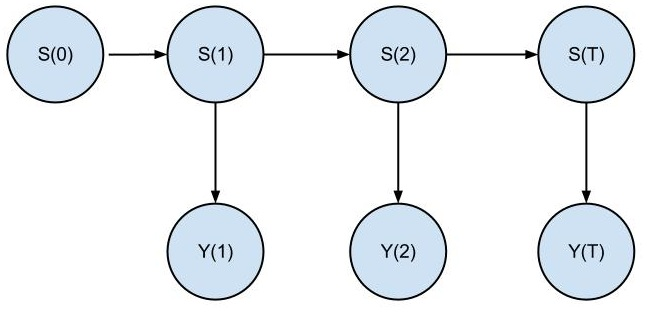
\includegraphics[width = .9\textwidth]{hmm}
  \hrule
  \caption{Hidden Markov Model}
  \label{hmm_figure}
\end{figure}



Training speaker dependent HMMs on isolated data from the sources to be separated, these models are then combined together in an architecture called factorial-max HMMs. The different HMMs evolve independently and for each observation vector produced at time t by each HMM, the elementwise maximum is chosen to create an observation. This is because the log magnitude spectrogram of a mixture of sources is very similar to the elementwise maximum of the individual spectrograms\footnote{This example was performed on two speakers. $a_{x_{t}}$ is the observation vector for speaker $x$ at time $t$, likewise is $b_{z_{t}}$ the observation vector for speaker $z$ at time $t$}. Separation is performed by setting the various masking signals to 1 or 0, depending on the observation vector at time $t$ for frequency band $i$.

\begin{figure}[h]
  \centering
  \hrule
  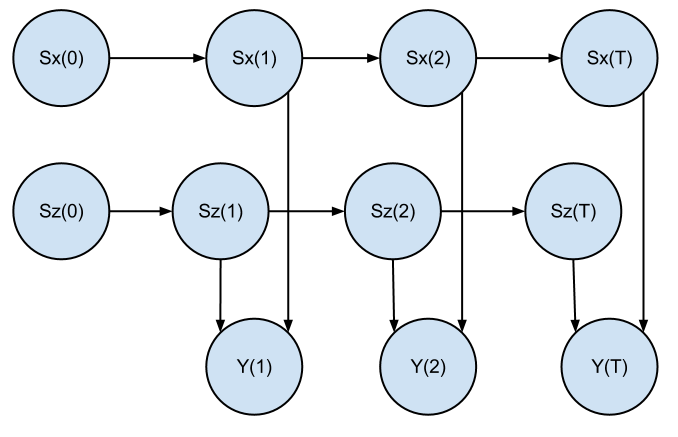
\includegraphics[width = .9\textwidth]{f_hmm}
  \hrule
  \caption{Factorial Hidden Markov Model}
  \label{fhmm_figure}
\end{figure}

The full generative model is given in Equations \ref{roweisEqn1} - \ref{roweisEqn3}.

\begin{equation}\label{roweisEqn1}
  p(x_{t}=j|x_{t-1}=i)=T_{ij}
\end{equation}

\begin{equation}\label{roweisEqn2}
  p(z_{t}=j|z_{t-1}=i)=U_{ij}  
\end{equation}

\begin{equation}\label{roweisEqn3}
  p(y_{t}|x_{t},z_{t})=N(max[a_{x_{t}},b_{z_{t}}], R)  
\end{equation}


\section{Conclusion}\label{conclusion}

In this survey we have provided an overview over some techniques in
blind source separation. Early work on blind source separation focused
to a large extent on time domain ICA. In extending the BSS problem to
multiple sources, the classical ICA method has been augmented by
adopting different signal representations, where the time-frequency
domain is particularly common. Different methods have also been
introduced, some borrowing from the human auditory system attempting
to hard-code domain specific knowledge. Others adopt different
algorithms; one important example here being hidden markov models
(HMMs). This is a very flexible approach to BSS as it allows for
non-stationary mixing, and relaxes many of the stringent assumptions
of classical ICA. 



\section{Research Agenda}\label{protocol}
The aim of this study is to systematically review current technology
for blind source separation (BSS), with particular emphasis on the
particular subproblem of single channel blind source separation
(SCBSS); that is, the recovery of several source signals from one observed signals.


\subsection{Background}
The blind source separation problem consists transforming a set of observed signals that has undergone some particular mixing process back to the original unobserved signals. The “blind” part of the problem refers to the fact that the nature of the mixing process is unknown. From original research on the blind source separation problem, focus has shifted from the case where with as many, or more recording channels than original sources, to the case of fewer channels than original sources. An important subproblem that we wish to focus on is where we have only one recording and attempt to recover multiple sources.

Our approach is two-fold: firstly we wish to look at studies about the performance of current single channel separation methods. Secondly, we wish to gain a broader overview over the state of research on BSS.

\subsection{Research Questions}
\begin{enumerate}
  \item What are the different variations on the blind source
    separation problem, in particular as pertains to audio data.
  \item Which methodologies and algorithms are applied to the
    different variations of the blind source separation problem as identified in Question 1.
  \item What are the theoretical properties of the techniques
    identified in Question 2, and  what assumptions do they make about the nature of the sources and the mixing process?
  \item What empirical evidence is there to document the performance
    of the techniques identified in Question 2 as applied to the
    problems identified in Question 1?
\end{enumerate}



\subsection{Search Strategy}
In reviewing the BSS literature we conduct a search of the below databases based on a set of keywords listed below. To filter the results we introduce a set of criteria to judge the relevance and quality of the results.

\subsubsection{Databases}

\begin{itemize}
 \item \href{www.springerlink.com}{SpringerLink}
 \item \href {www.citeseerx}{CiteSeerX}
 \item \href{scholar.google.com}{Google Scholar}
\end{itemize}

\subsubsection{List of Search Terms}

\emph{blind source separation, single channel blind source separation, single mixture blind source separation, hidden markov blind source, single microphone blind source separation, blind source separation review, blind source separation survey, pca blind source separation, ica blind source separation, principal component analysis blind source separation, independent component analysis blind source separation}.



\subsubsection{Inclusion and Quality Criteria}
We wish to study how various methods and/or approaches by which blind source problem is solved, which constraints are imposed by these methods, and how well a BSS system based on these ideas perform on real-life data. To filter out the most important studies to this end, we adopt the following criteria.

\begin{description}
	\item Inclusion Criteria
		\begin{enumerate}
			\item The main concern of the study is the BSS
                          problem.
			\item The algorithmic design decisions in the study must be justified.
			\item The study describes a reproducible algorithm/method.
			\item The study focuses on blind source separation of auditory signals.
		\end{enumerate}
	\item Quality Criteria
		\begin{enumerate}
			\item The study presents empirical results.
			\item More recent studies are preferred.
			\item The described test data set is
                          reproducible.
                        \item The study should present novel
                          theoretical approaches/methodologies OR
                          empirical results about previously known methods. 
			\item Literature reviews should discuss single channel blind source separation.
			\item The study should describe which other algorithms/methods the proposed solution can be compared with and the performance measure used in comparison.
		\end{enumerate}
\end{description}








\chapter{Principal Component Analysis}\label{pca}

Principal component analysis \cite{pearson1901} (PCA) is a eigenvector-based,
non-probabilistic technique that uses orthogonal projection to
represent data in a lower dimensional subspace spanned by the $k$
first eigenvectors of the covariance matrix. The eigenvectors form an
orthogonal basis for the data such that a projection onto the
eigenvectors will decorrelate the data. In the next section we will
derive this result by maximizing the variance of an axis of
projection.


PCA is useful in several applications, hereunder visualization and
detection of so-called \emph{latent variables}. The principal
components (PCs) are the basis of the subspace onto which the data is
projected, and are such that the variance explained by each component
is maximized; that is, the first PC explains a higher proportion of
variance than the second PC and so forth. We can therefore, by
retaining only the first few components acheive a representation of
the data containing the most of the variance exhibited by the
assumption that the PCs accounting for the smallest portion of
variance are noise.


The next sections presents PCA from two different but equivalent
perspectives; Secion \ref{pca_intuition} presents some intuition
behind PCA and how we use projections to reduce
dimensionality\footnote{It should be noted that while in many
  applications of PCA, dimenension reduction is the main aim, in
  direct applications of  PCA to source separation, we are more
  interested in the fact that the projected data is uncorrelated.} in data
so as to make it simple to capture the distinctive features of the
phenomenon we are interested in. We then proceed more
analytically, first solving for the direction of maximal variation
using the method of Lagrange multipliers, and subsequently by singular
value decomposition. The latter is the more computationally
efficient, and the rationale for this approach is easy to see once the
first perspective is known. We then proceed to looking at how PCA can
be applied to the blind source problem and how the assumptions made
about the data affect the results of a real-world mixing case.


\section{Intuition}\label{pca_intuition}

Consider the two dimensional dataset of Figures
\ref{pca1}-\ref{pca2}. We now want to find a new
\emph{one-dimensional} representation for
this data that captures the most of the variation in this data. Figures
\ref{pca1}-\ref{pca2} illustrate two attempts at doing this by drawing
twostraight lines through the set of points. Notice the difference
between the two lines; as the line in Figure \ref{pca1} runs
almost perfectly through the points, there are only three points that
differ significantly from the others which lie almost on the line. As for
the line in Figure \ref{pca2}, we can distinguish between most of the
points by virtue of their distance from the line\footnote{ While we may not
guarantee that this particular line will serve as well with future
points, we can at least say it does a good job with the limited sample
we have.}.

\begin{figure}
  \centering
  \hrule
  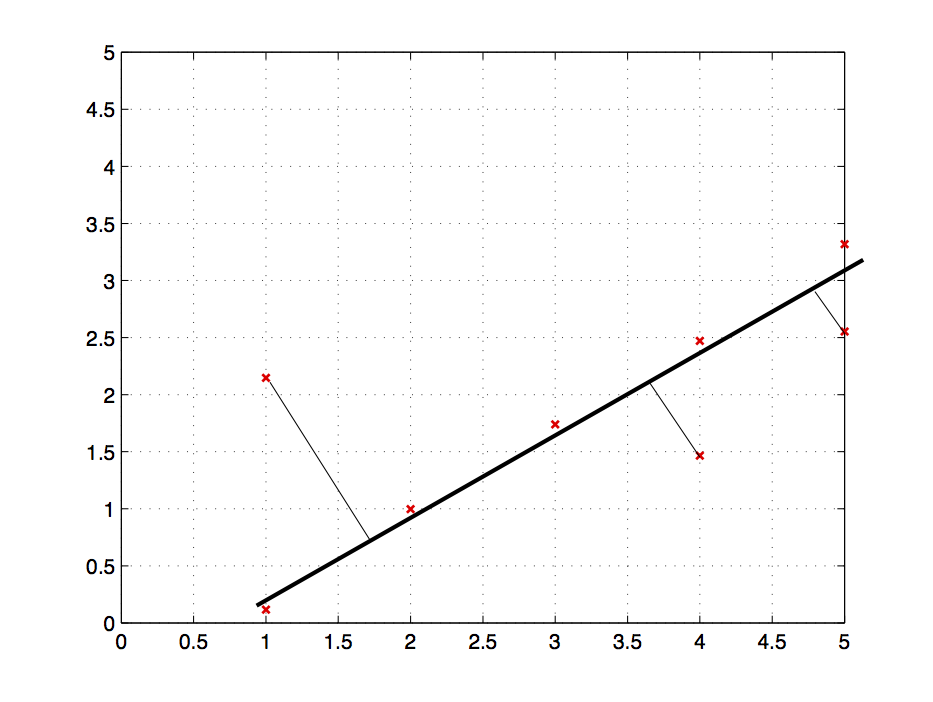
\includegraphics[width = .9\textwidth]{Figures/pca1.png}
  \hrule
  \caption{After projecting the data onto the dark line, little
    variation left in the dataset.}
  \label{pca1}
\end{figure}

Now we want to introduce some terminology so we may extend our
intuition to more complex (and realistic cases). In the example above,
each of our original data points are \emph{vectors} $\mathbf{v}_i$ in two
dimensional Euclidean space $\mathbb{R}^2$. The dimensionality
reduction operation is here a projection $T:
\mathbb{R}^2\rightarrow\mathbb{R}$. In the general case of PCA we are
interested in finding such projections $T:
\mathbb{R}^m\rightarrow V$ to maximize the variance of the data
projected onto a lower dimensional vector space $V$.


We characterize a vector space $V$ by its \emph{basis} $B=\{\mathbf{u}_1,...,\mathbf{u}_N\}$, which is a set
of vectors such that any vector $\mathbf{v}\in V$ can be expressed as a linear
combination of $B$. The projection operation discussed above can be
thought of as a change of basis. In the context of Figure \ref{pca2}
the new basis may be a vector $\mathbf{u} = (1,-1)^T$. $\mathbf{u}$
would then correspond to a unit vector in the direction of the dark line. For any point $\mathbf{x}_i =
(x_i^{(1)}, x_i^{(2)})^T$, the only operation we need to express it in the new
basis is computing the dot product $\mathbf{u}\cdot \mathbf{x}_i$.


\begin{figure}
  \centering
  \hrule
  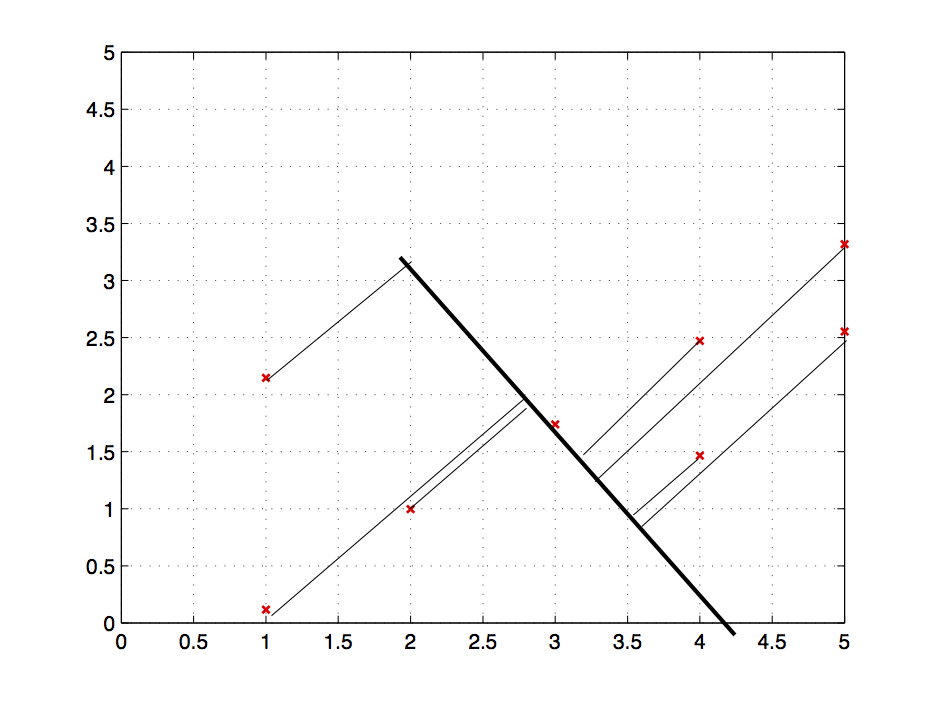
\includegraphics[width = .9\textwidth]{Figures/pca2.png}
  \hrule
  \caption{Projecting the data onto the dark line we reduce
    dimensionality while keeping a large portion of the variation
    characterizing the data.}
  \label{pca2}
\end{figure}

In the next sections we will formalize these ideas and look at how we
actually compute the bases $B$ so as to find the axis of maximum
variability for a given dimensionality. 

\section{Formal Statement}

In this section we review the PCA problem as a constrained
maximization problem. We seek to maximize the variance of the
projected data by means of the method of Lagrange multipliers. 


Let $\boldsymbol{x}_i \in \mathbf{R}^n$ denote the $i$'th observation of a dataset
of $m$ observations. We now want to project our data onto a vector $\boldsymbol{u}$
in $\mathbb{R}^n$ so as to maximize the variance of the resulting
projection $\sum_{i=1}^m \boldsymbol{x}_i^T \boldsymbol{u}$ subject to the constraint
$|\boldsymbol{u}|=1$. Under the assumption that $\boldsymbol{X}$ is
standardized to zero mean and unit variance, the Lagrangian is then
given by Equation \ref{pca_lagrangian}:


  \begin{equation}
    \label{pca_lagrangian}
    \begin{array}{lcl}
      \mathcal{L}(u,\lambda) & = & \frac{1}{m} \sum_{i=1}^m (\boldsymbol{x}_i^T \boldsymbol{u})^2 - \lambda (\boldsymbol{u}^T \boldsymbol{u} -1) \\
      \\& = & \frac{1}{m} \sum_{i=1}^m (\boldsymbol{u}^T \boldsymbol{x}_i)^T(\boldsymbol{x}_i^T \boldsymbol{u}) - \lambda (\boldsymbol{u}^T \boldsymbol{u} -1) \\
      \\& = & \frac{1}{m} \sum_{i=1}^m \boldsymbol{u}^T(\boldsymbol{x}_i \boldsymbol{x}_i^T)u - \lambda (\boldsymbol{u}^T \boldsymbol{u} -1) \\
      \\& = & \frac{1}{m}  u^T\sum_{i=1}^m(\boldsymbol{x}_i \boldsymbol{x}_i^T)\boldsymbol{u} - \lambda (\boldsymbol{u}^T \boldsymbol{u} -1) \\
      \\& = & \frac{1}{m} \boldsymbol{u}^T \boldsymbol{\Sigma} \boldsymbol{u} - \lambda (\boldsymbol{u}^T \boldsymbol{u} -1) \\
    \end{array}
  \end{equation}

Here, $\boldsymbol{\Sigma} = \sum_{i = 1}^m \boldsymbol{x}_i
\boldsymbol{x}_i^T$ is the covariance matrix. Setting the gradient of
\ref{pca_lagrangian} equal to zero yields Equation \ref{pca_gradient}:


\begin{equation}
  \label{pca_gradient}
  \nabla_u \mathcal{L}(\boldsymbol{u}, \lambda) = \boldsymbol{\Sigma} \boldsymbol{u} - \lambda \boldsymbol{u} = 0
\end{equation}

Equation \ref{pca_gradient} shows that the direction of maximum
variance $u$, which we will refer to as the first principal component,
is the first eigenvector of the covariance matrix of the dataset. By
similar means it can be shown that the second eigenvector points in
the direction of largest variance \emph{orthogonal} to the first
eigenvector and so forth. Finally it is worth noting that the portion
of the total variance explained by a principal component is
proportional to its associated eigenvalue.


\subsection{Singular Value Decomposition}

For a high dimensional dataset (e.g. $n = 10,000$), which is
frequently the case working with for instance image or video data, the
covariance matrix will have $10,000\times 10,000 = 100,000,000$
entries, which is computationally untractable. Hence, PCA is usually
implemented in terms of \emph{singular value decomposition} (SVD). For
an $m\times n$ matrix $\boldsymbol{X}$, the SVD is a factorization
such that:


\begin{equation}
  \boldsymbol{X} = \boldsymbol{USV}^{T}
\end{equation}


Here, $\boldsymbol{U} \in \mathbb{R}^{m\times m}$, $\boldsymbol{S} \in \mathbb{R}^{m\times n}$,
and $\boldsymbol{U} \in \mathbb{R}^{n\times n}$. The SVD relates to the eigenvalue
problem (Equation \ref{pca_gradient}) as follows:


\begin{itemize}
\item The columns of $\boldsymbol{U}$ form the projections of $\boldsymbol{X}$ onto the
  eigenvectors $\boldsymbol{V}$.
  \item The entries $s_{ii}$ on the leading diagonal of $\boldsymbol{S}$ are the
    eigenvalues of $\boldsymbol{\Sigma} = \boldsymbol{X}^T\boldsymbol{X}$.
  \item The top $k$ columns of $\boldsymbol{V}$ are the top $k$ eigenvectors of
    $\Sigma = \boldsymbol{X}^T \boldsymbol{X}$
\end{itemize}


Most statistics libraries provide SVD functionalities that are highly
optimized, hence we will not cover algorithms for computing the SVD
here\footnote{In \textsc{Matlab}, we can perform SVD using the
  \texttt{svd}
statement: \texttt{[u,S,v] = svd(X)}.}.


We will not go into the derivation of this result as SVD is covered
in most textbooks on linear algebra or basic numerical
mathematics (see for instance REF). Rather, we will proceed to show how PCA can be applied to
BSS, and what assumptions it requires us to make about the data.




\section{PCA Application to Blind Source Separation}\label{pca_bss}




We have so far looked at PCA as a method of transforming data from
$N$-dimensional Euclidean space onto a set of \emph{principal components}
which is the basis of a new vector space $\boldsymbol{V}$. A key property of $\boldsymbol{V}$ is
that the data is now linearly uncorrelated. This is in turn the key
idea to take into account in blind source separation.

The top graph of Figure \ref{pca_time_series} shows two periodic
signals $s_1$ and $s_2$ contaminated by an additive Gaussian white
noise with standard deviation $\sigma = .2$.


\begin{equation}
      \begin{array}{lll}
        s_1 = & \sin(\pi x) & 0<x<5\\
        s_2 = & \cos(7 \pi x) & 0<x<5\\
    \end{array}
\end{equation}

The signals are subsequently mixed, as shown in the middle part of
Figure \ref{pca_time_series} by the matrix:


\begin{equation}
  \boldsymbol{A} = \begin{bmatrix} \cos \alpha & -\sin \alpha \\ \sin \alpha & \cos \alpha \end{bmatrix}
\end{equation}

where $\alpha = \pi/4$. Here the mixing matrix $\boldsymbol{A}$ corresponds to a
rotation operator that will rotate the data by $\alpha$ radians in
counterclockwise direction. 


The lower part of Figure \ref{pca_time_series} shows the recovered
signal\footnote{The estimated unmixing matrix here is $\hat{W} =
  \hat{A}^{-1} = \begin{bmatrix} .7071 & .7071 \\ -.7071 &
    .7071 \end{bmatrix}$ which is, as expected, the inverse of $A$ for
  the value of $\alpha$ above.}.


\begin{itemize}
  \item Example where it works - why
  \item Example where it fails - why
\end{itemize}



\begin{figure}
  \centering
  \hrule
  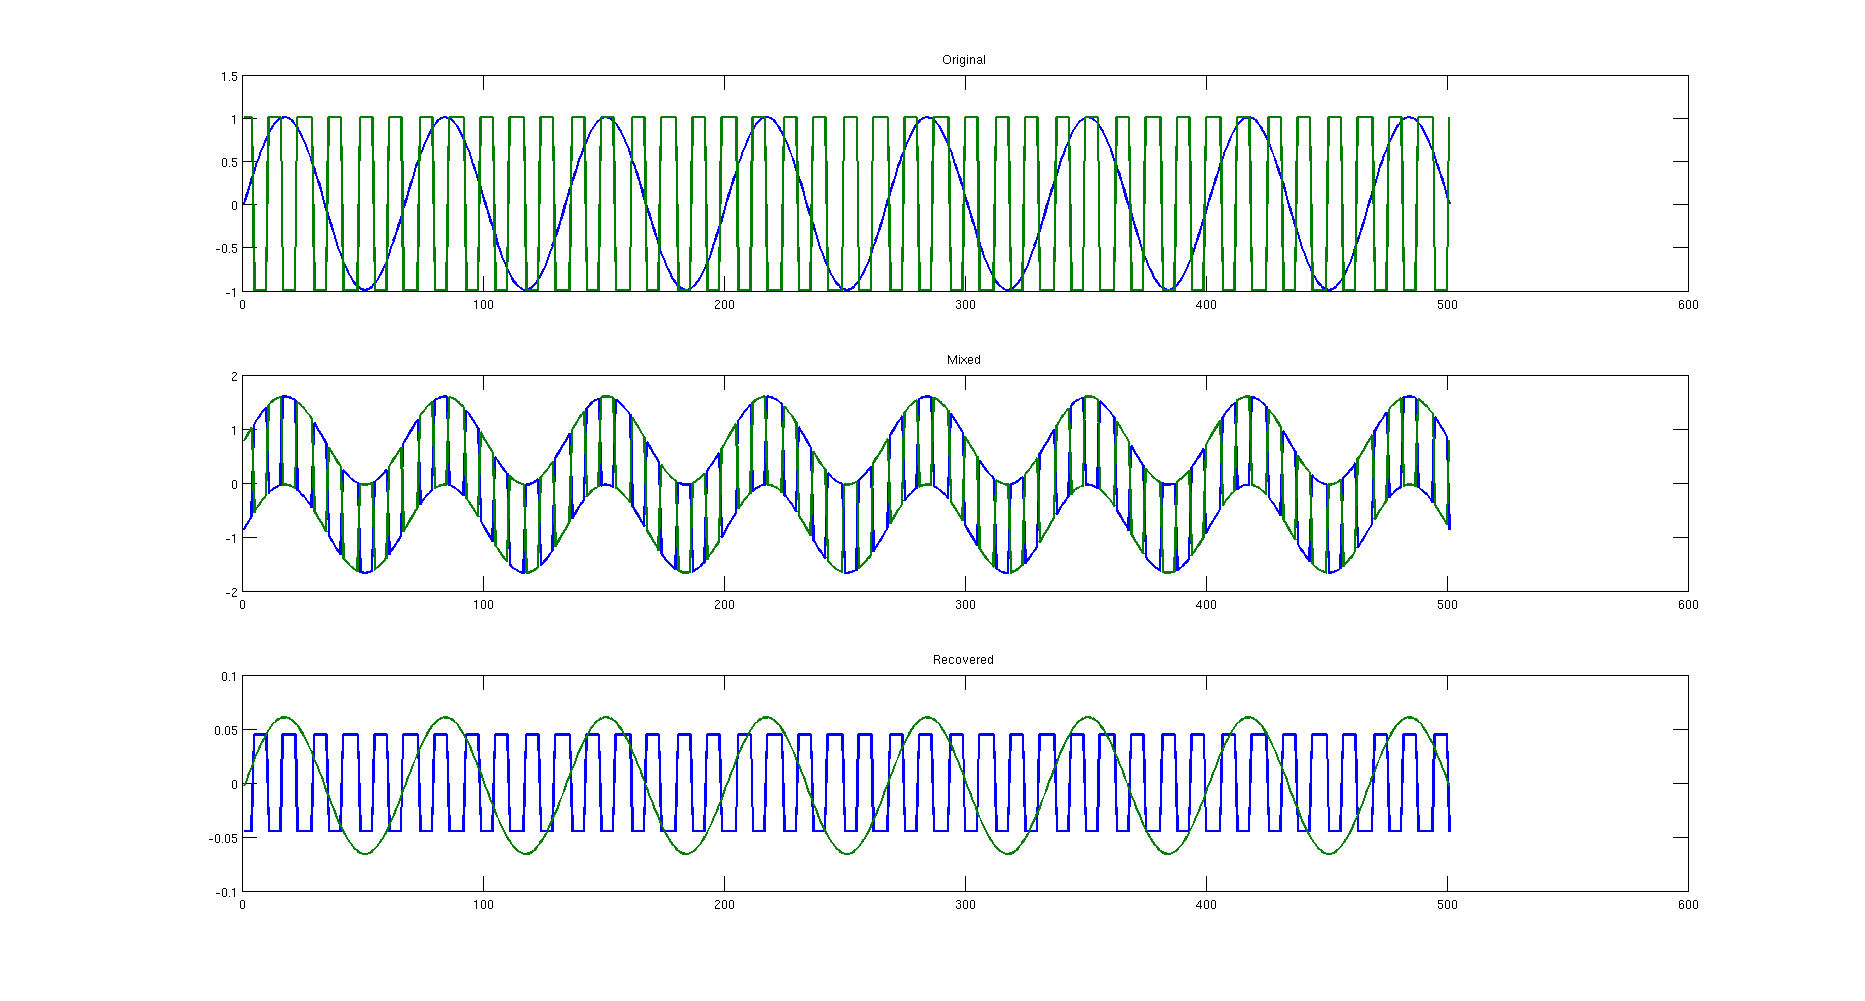
\includegraphics[width = .9\textwidth]{Figures/pca_signal_time_series}
  \hrule
  \caption{PCA Source Separation.}
  \label{pca_time_series}
\end{figure}

\begin{figure}
  \centering
  \hrule
  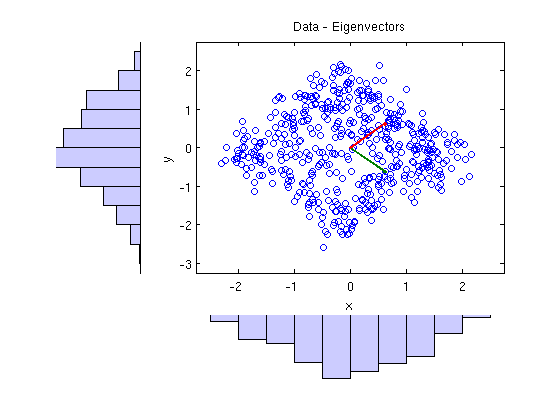
\includegraphics[width = .9\textwidth]{Figures/pca_data_eigs}
  \hrule
  \caption{Standardized data points vs eigenvectors.}
\end{figure}

\begin{figure}
  \centering
  \hrule
  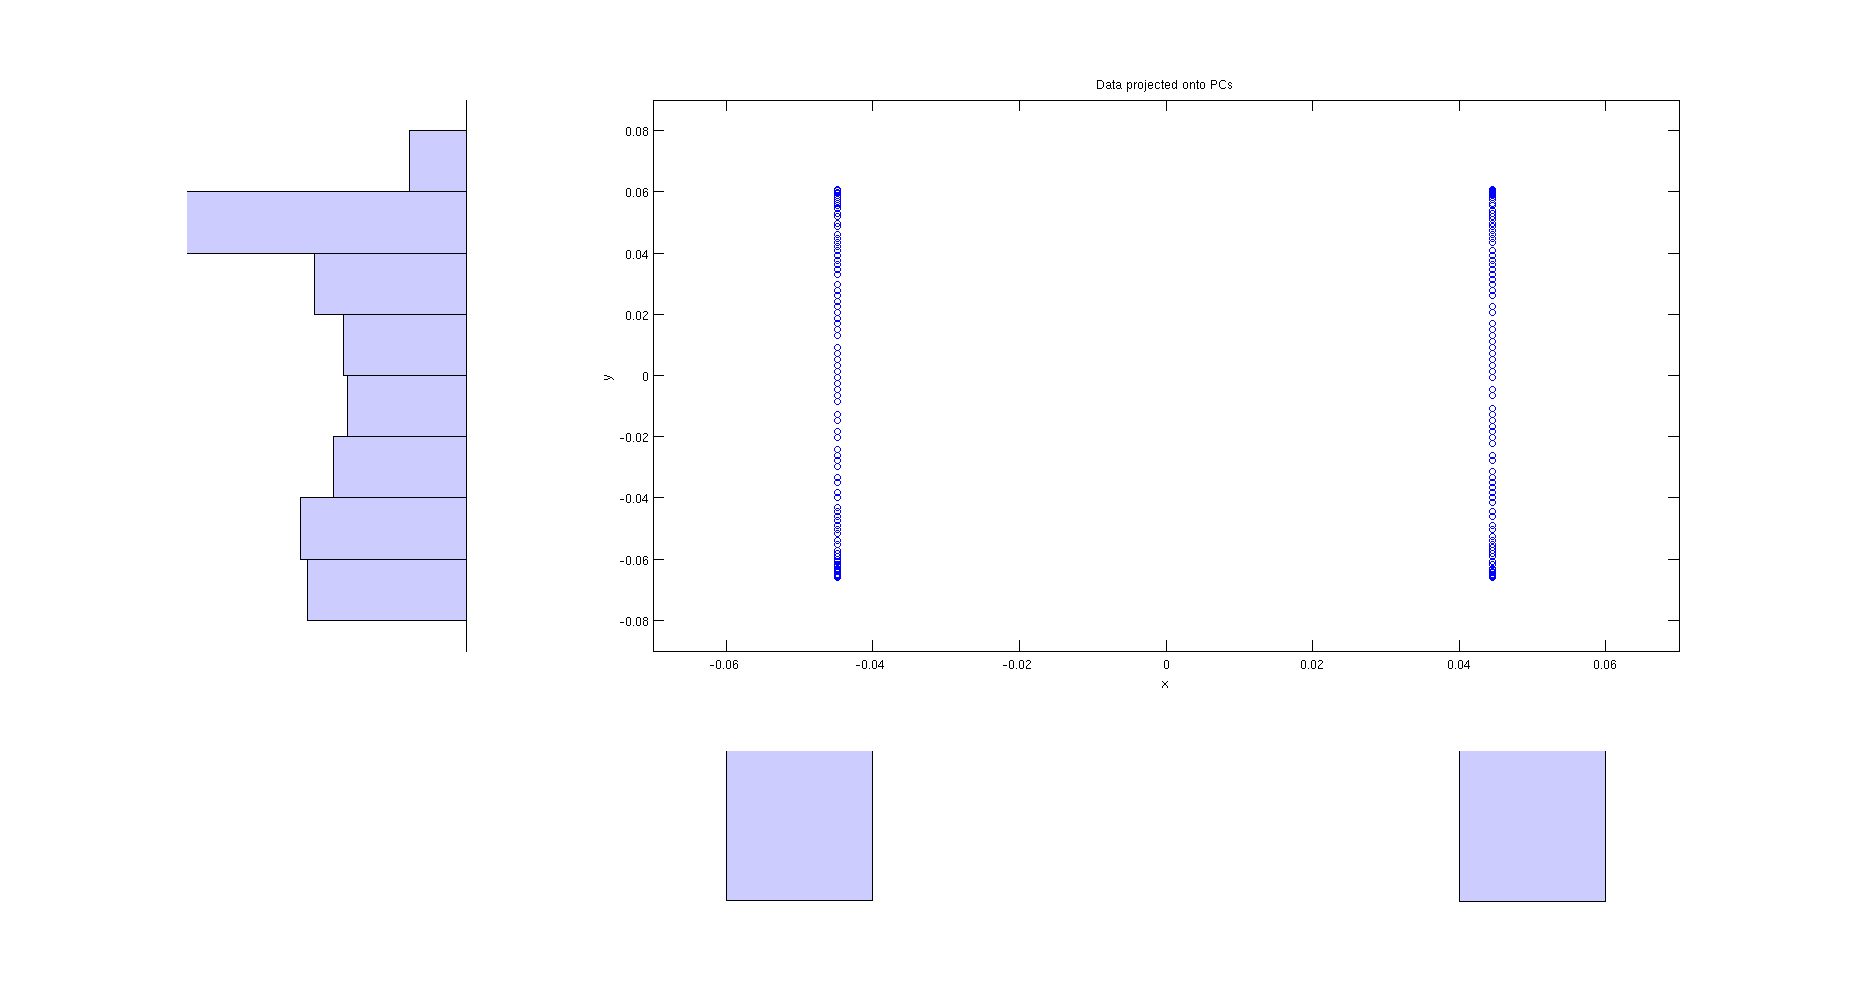
\includegraphics[width = .9\textwidth]{Figures/pca_eig_projection}
  \hrule
  \caption{Standardized data projected onto eigenvectors.}
\end{figure}





\chapter{Independent Component Analysis}\label{ica}


PCA finds the basis of a subspace in which the variance is
maximized in the direction of the basis vectors and the covariance
between the data is zero. ICA seeks to find basis
vectors that are statistically independent, which is a stronger
property than simply being uncorrelated as independence implies
uncorrelatedness, while the opposite is not true. 
Like PCA, we can interpret ICA as an optimization problem, but in
contrast to PCA, ICA does not have a general closed form solution, 
so a numerical optimization method is usually applied in
computing the ICA transform.

This chapter is structured as follows. First we give a brief overview
over different approcahes to ICA in Section \ref{equiv_ica}. We then 
consider some limitations of the ICA model in Section \ref{ICA_restrictions}, 
with particular emphasis on the non-gaussianity constraint, which is 
important with respect to the types of data we can analyze using ICA. Section 
\ref{linear_model_ica} goes into the maximum likelihood approach to ICA in 
further detail, and derives a gradient descent learning rule for independent
components analysis. As it turns out, this gradient rule is similar to the 
learning rules proposed under the different frameworks discussed in 
Section \ref{equiv_ica}. Finally, Section \ref{bss_ica} illustrated ICA 
with a few blind source separation problems.


\section{Equivalent Statements of ICA}\label{equiv_ica}

ICA can be derived by several different approaches representing slightly
different interpretations of the same problem. Among these are maximum 
differential entropy (REFFFF), maximum kurtosis (REF) and 
maximum likelihood (\cite{Pham}). 
In this section we provide a brief overview over the two first, while we
go in more detail on the maximum likelihood method in subsequent sections.

\subsection{Kurtosis Maximization}

The kurtosis $\beta_X$ of a random variable $X$ is defined as the fourth
moment around the mean $\mu_X$:


\begin{equation}
  \beta_X = \frac{\mathbb{E}[(X-\mu_X)^4]}{\mathbb{E}[(X-\mu_X)^2]^2} 
\end{equation}

If we standardize our data to zero mean and unit variance, we see that
the above simplifies to $\mathbb{E}(X^4)$. Often times, we are
interested in comparing a distributions to the normal distribution by
means of kurtosis, which leads to the definition of \emph{excess
  kurtosis}, $\gamma = \beta - 3$, where the $-3$ term is necessary to
make the kurtosis of the normal distribution zero. 

We now consider the problem $\boldsymbol{x}=\boldsymbol{A}\boldsymbol{x}$ 
and let $\boldsymbol{W} = \boldsymbol{A}^{-1}$. Setting 
$\hat{\boldsymbol{s}} = \boldsymbol{W}^T\boldsymbol{x}$, and
$\boldsymbol{z} = \boldsymbol{A}^T\boldsymbol{W}$, we can substitute into
the equation for $\hat{\boldsymbol{s}}$:


\begin{equation}
  \hat{\boldsymbol{s}} = \boldsymbol{W}^T\boldsymbol{x} = \boldsymbol{W}^T\boldsymbol{A}\boldsymbol{s}
  =\boldsymbol{z}\boldsymbol{s}
\end{equation}

We now rely on the following property of kurtosis 
$\gamma(ax_1+bx_2) = a^4\gamma(x_1) + b^4\gamma(x_2)$, and note that as 
$\boldsymbol{z}$ is a square matrix of the same dimension as the mixing 
matrix\footnote{We assume that there is an equal number of sources as observables.},
$\boldsymbol{z}\boldsymbol{s}$ is of the same dimension as the as the input. 
The kurtosis of the estimate $\hat{\boldsymbol{s}}$ is the weighted product
of the columns of $\boldsymbol{z}\boldsymbol{s}$:


\begin{equation}
  \label{kurtosis_eqn}
  \gamma(\hat{\boldsymbol{s}}) = \gamma(\boldsymbol{z}\boldsymbol{s})
  = \sum_{i=1}^N \boldsymbol{z}_i^4\gamma(\boldsymbol{s}_i)
\end{equation}

(Equation \ref{kurtosis_eqn}) lends itself easily to standard optimization
procedures to maximize kurtosis so as to produce the independent components:

\begin{equation}
  \boldsymbol{s}_i = \arg \max_{s_i} \sum_{i=1}^N \boldsymbol{z}_i^4\gamma(\boldsymbol{s}_i)  
\end{equation}

Kurtosis maximization is of the most common approaches to ICA and is discussed
in greater detail in REFERANSER!!!.


\subsection{Minimum Mutual Information}

The differential entropy $H$ of a random variable $Y$ with density $g(y)$ is given by:
\begin{equation}
  H(Y) = - \int g(y) \log g(y) dy
\end{equation}

The mutual information, $I(Y)$, between the components of the the random vector $Y$ is a natural measure of dependence:

\begin{equation}
  I(Y) = \sum_{j=1}^{p} H(Y_{j}) - H(Y)
\end{equation}

The sum $I(Y)$ is the \emph{Kullback-Leibler distance} between the density $g(y)$ of $Y$ and its independence 
version $\prod_{j=1}^{p} g_{j}(y_{j})$, where $g_{j}(y_{j})$ is the marginal density of $Y_{j}$. The ICA of a random 
vector $\mathbf x$ can be defined as a invertible transformation where the matrix $\mathbf A$ is determined 
so that the mutual information of the transformed components $s_i$ is minimized.
An important property of mutual information is that if we have an invertible linear transformation 
$y = \mathbf Ax$ then:

\begin{equation}\label{determinant}
I(Y) = \sum_{j=1}^{p} H(y_{j}) - H(x) - \log | det \mathbf A |
\end{equation}

Determining an $\mathbf A$ to minimize $I(Y) = I(\mathbf A^T \mathbf x)$ is the looks for the orthogonal 
transformation that maximizes independence between its components $s_i$. With respect to 
(Equation \ref{determinant}), this is equivalent to minimizing the sum of entropies of the seperate 
components of $Y$ which maximizes their depature from Gaussianity.




\section{Limitations of the ICA Model}\label{ICA_restrictions}

ICA imposes a few critical assumptions about the nature of the sources
and the extentent to which they can be recovered. In short, these are:


\begin{itemize}
  \item \emph{Signal ordering}: We cannot recover the correct order of
    the signals.
  \item \emph{Scaling}. Recovered signals may be scaled arbitrarily.
  \item \emph{Gaussianity}. We cannot recover Gaussian sources.
\end{itemize}


As in PCA, we cannot
recover the original ordering of the signals; i.e. the rows of the
source matrix $\boldsymbol{S}$ may be swapped in the resulting
$\hat{\boldsymbol{S}}$. Furthermore, the correct scaling of the source
compents, including their sign cannot be recovered. This can be seen
in that $\boldsymbol{X} = \boldsymbol{A}\boldsymbol{S} = (.5
\boldsymbol{A})(2 \boldsymbol{S})$.

The final limitation of ICA is that the source signals must be
non-Gaussian. To see why this must hold, we rely on the fact that the
multivariate gaussian distribution is rotationally symmetric. Furthermore,
to fully recover the sources, we must be able to ``undo'' any rotation
caused by applying the mixing operator. To see the effect of an
applying a rotation operator to a sine wave, consider the example in
Section \ref{pca_bss}.

Consider a single observation
$\boldsymbol{x} = \boldsymbol{x}(t) =\boldsymbol{A}\boldsymbol{s}(t) =
\boldsymbol{A}\boldsymbol{s}$. The covariance matrix of
$\boldsymbol{x} = \boldsymbol{A}\boldsymbol{s}$ is:


    \begin{equation}
      \mathbb{E}(\boldsymbol{x}\boldsymbol{x}^T) 
      = \mathbb{E}((\boldsymbol{A}\boldsymbol{s})(\boldsymbol{A}\boldsymbol{s})^T) = \mathbb{E}(\boldsymbol{A}\boldsymbol{s}\boldsymbol{s}^T\boldsymbol{A}^T)=\boldsymbol{A}\boldsymbol{A}^T      
    \end{equation}

Now, let $\boldsymbol{R}$ be a rotation operator and $\boldsymbol{A}'
= \boldsymbol{AR}$. We consider mixing $\boldsymbol{s}$ by
$\boldsymbol{A}'$ instead. The covariance matrix of  
$\boldsymbol{x}' = \boldsymbol{A}'\boldsymbol{s}$ is:


\begin{equation}
  \begin{array}{lcl}
    \mathbb{E}(\boldsymbol{x}'\boldsymbol{x}'^T) & = &
    \mathbb{E}((\boldsymbol{A}'\boldsymbol{s})(\boldsymbol{A}'\boldsymbol{s})^T) \\
    \\& = & \mathbb{E}(\boldsymbol{A}'\boldsymbol{s}\boldsymbol{s}^T\boldsymbol{A}'^T) \\
    \\& = & \mathbb{E}(\boldsymbol{A}\boldsymbol{R}\boldsymbol{s}\boldsymbol{s}^T(\boldsymbol{A}\boldsymbol{R})^T) \\
    \\& = & \boldsymbol{A}\boldsymbol{R}\boldsymbol{R}^T\boldsymbol{A}^T
    \\& = & \boldsymbol{A}\boldsymbol{A}^T
  \end{array}
\end{equation}

Hence, we see that both $\boldsymbol{s}$ and $\boldsymbol{s}'$ come
from the same Gaussian distribution $\boldsymbol{\Phi}(0,
\boldsymbol{A}\boldsymbol{A}^T$). This means that the recovered data
may be rotated by an arbitrary rotation matrix $\boldsymbol{R}$, which
as discussed above, provides little information about the sources. 


\section{Maximum Likelihood ICA in the Linear Mixing Model}\label{linear_model_ica}

INTRO BS....

Consider the value of a single source $s_i$ at a given instant in time, and
let $p_s(s_i)$ be the probability density function for source $i$. Assuming the 
sources are independent the joint distribution of all the $n$ sources is given 
by the product of the marginal distributions of each source:

\begin{equation}
  p_s(s) = \Pi_{i=1}^n p_s(s_i)
  \label{ica_prob}
\end{equation}

Recalling our notation for the unmixing model:

\begin{equation}
  \boldsymbol{A}^{-1} = \boldsymbol{W} = 
  \begin{bmatrix} 
    \boldsymbol{w}_1^T\\ \boldsymbol{w}_2^T\\ ...\\ \boldsymbol{w}_n^T\\
  \end{bmatrix}
\end{equation}

We can substitute for $s_i$ in (Equation \ref{ica_prob}), to obtain the following
expression for the joint distribution\footnote{Here the determinant term results from
the rule for linear transformations of probability densities.}.

\begin{equation}
    p(s) = \Pi_{i=1}^n p_s(\boldsymbol{w}_i^T \boldsymbol{x}) \cdot |\boldsymbol{W}|    
\end{equation}


Under maximum likelihood estimation, we want to find the $\boldsymbol{W}$ that is most likely given our 
dataset $\boldsymbol{X} = [\boldsymbol{x}_1,\boldsymbol{x}_2,...,\boldsymbol{x}_T]$, ie.


\begin{equation}
  \label{max_likelihood}
  \boldsymbol{W}^* = \arg \max_{\boldsymbol{W}} \mathbb{P}(\boldsymbol{W}|\boldsymbol{X})
\end{equation}

By straight forward application of Bayes' rule, we can rewrite the probability in (Equation \ref{max_likelihood}) as:

\begin{equation}
  \label{bayes}
  \mathbb{P}(\boldsymbol{W}|\boldsymbol{X}) 
  = \frac{\mathbb{P}(\boldsymbol{X}|\boldsymbol{W}) \mathbb{P}(\boldsymbol{W})}{\mathbb{P}(\boldsymbol{X})}
  \propto \mathbb{P}(\boldsymbol{X}|\boldsymbol{W})
\end{equation}

From (Equation \ref{bayes}), we can set up the maximum likelohood function:

\begin{equation}\label{ica_loglikelihood}
  \begin{array}{lll}
    l(W) & = &\log \mathbb{P}(\boldsymbol{X}|\boldsymbol{W}) \\
    & = & \Sigma_{t=1}^T \log p_s(\boldsymbol{W}\boldsymbol{X})+\log |\boldsymbol{W}|\\
    & = & \Sigma_{t=1}^T\Sigma_{i=1}^N\log p_s(\boldsymbol{w}_i^T\boldsymbol{x}(t)+\log |\boldsymbol{W}|
  \end{array}
\end{equation}

The final step is to determine the marginal distributions $p_s$ of the sources. 
A common, but not necessary assumption is to let all the sources have the same distribution.
As gaussian marginals are precluded by the assumptions of our model, we need to choose an
alternative distribution for $s$. Typically, the distribution is specified in terms of the 
cumulative density function $P_s(s)$. Standard choices here include the sigmoid 
$P_s(s) = \frac{1}{1+e^{-s}}$ and hyperbolic tangent ($P_s(s) = \tanh(s)$). 

\subsection{A Gradient Descent Rule for ICA}

Given the log likelihood function of Equation \ref{ica_loglikelihood},
we will now discuss how this can be maxmimized by gradient descent. 
The gradient descent method has an intuitive appeal, and  
lends itself easily to a computer implementation along the lines of
the pseudocode Figure \ref{ica_listing}. 

Gradient descent is an iterative optimization method where local extrema are found
by taking steps proportional to the gradient of the function at a given point. 
The algorithm may be seeded randomly or initialized by domain knowledge of the 
optimization problem at hand. Normally, the step size of the algorithm is decremented
as the algorithm converges, which is expressed through the learning rate $\alpha(n)$
which is a function of the current of iteration count $n$. We can state this as the following
update rule:


\begin{equation}
  \label{gradient_descent}
  x_{n+} = x_n + \alpha(n)\nabla F(x_n)
\end{equation}

The rule in (Equation \ref{gradient_descent} is iterated until convergence is reached.
This is typically measured by the difference $|x_{n+1}-x_n$ or in terms of the number of
iterations passed as in Figure \ref{mlica_code}.

In the particular case of objective functions that are the sum of a large number
of terms it is often convenient to apply a modified version of gradient descent
known as stochastic gradient descent, where only a randomly selected subset of the 
terms are computed in evalutating the gradient. Of the most important applications of this
rule is of course the maximization of log likelihood functions.

\begin{figure}[!htpb]\label{ica_listing}
  \begin{lstlisting}[frame=single]
% Variables:
X % Mixed sources
a % learning rate
w % unmixing matrix

for i = 1:nIter
  s = randomSubset(X)
  w = w + a*(1-2*(1/exp(-s))*s')*w;  
  \end{lstlisting}
  \caption{Pseudocode for ML ICA by stochastic block gradient descent.}
  \label{mlica_code}
\end{figure}

To conclude this section, we review the gradient descent algorithm of Figure \ref{mlica_code}.
Here, we assume the data is distributed according to a sigmoid cdf $f$. By inserting substituting
this into (Equation \ref{ica_loglikelihood}) and differentiating, we get the following update rule:


\begin{equation}
  \mathbf{W}_{n+1} = \mathbf{W}_{n} + \alpha(1-2*f(\mathbf{W}\mathbf{X})\mathbf{X}^T + (\mathbf{W}^T)^{-1})
\end{equation}

For a more sophisticated ICA algorithm, we refer to Hyvarinen's FastICA [REF].


\section{BSS by ICA}\label{BSS_ICA}

Here we also observe that the sign of the original speech signal is reversed in the 
bottom right recovered signal


\begin{figure}\label{ica_fig1}
  \centering
  \hrule
  \includegraphics[width = .9\textwidth]{Figures/ica_simple}
  \hrule
  \caption{ICA on a $2\times 2$ BSS problem. Note the ``sign reversal'' for the 
    blue sine wave (cf. Section \ref{ICA_restrictions}).}
\end{figure}

\begin{figure}\label{ica_fig2}
  \centering
  \hrule
  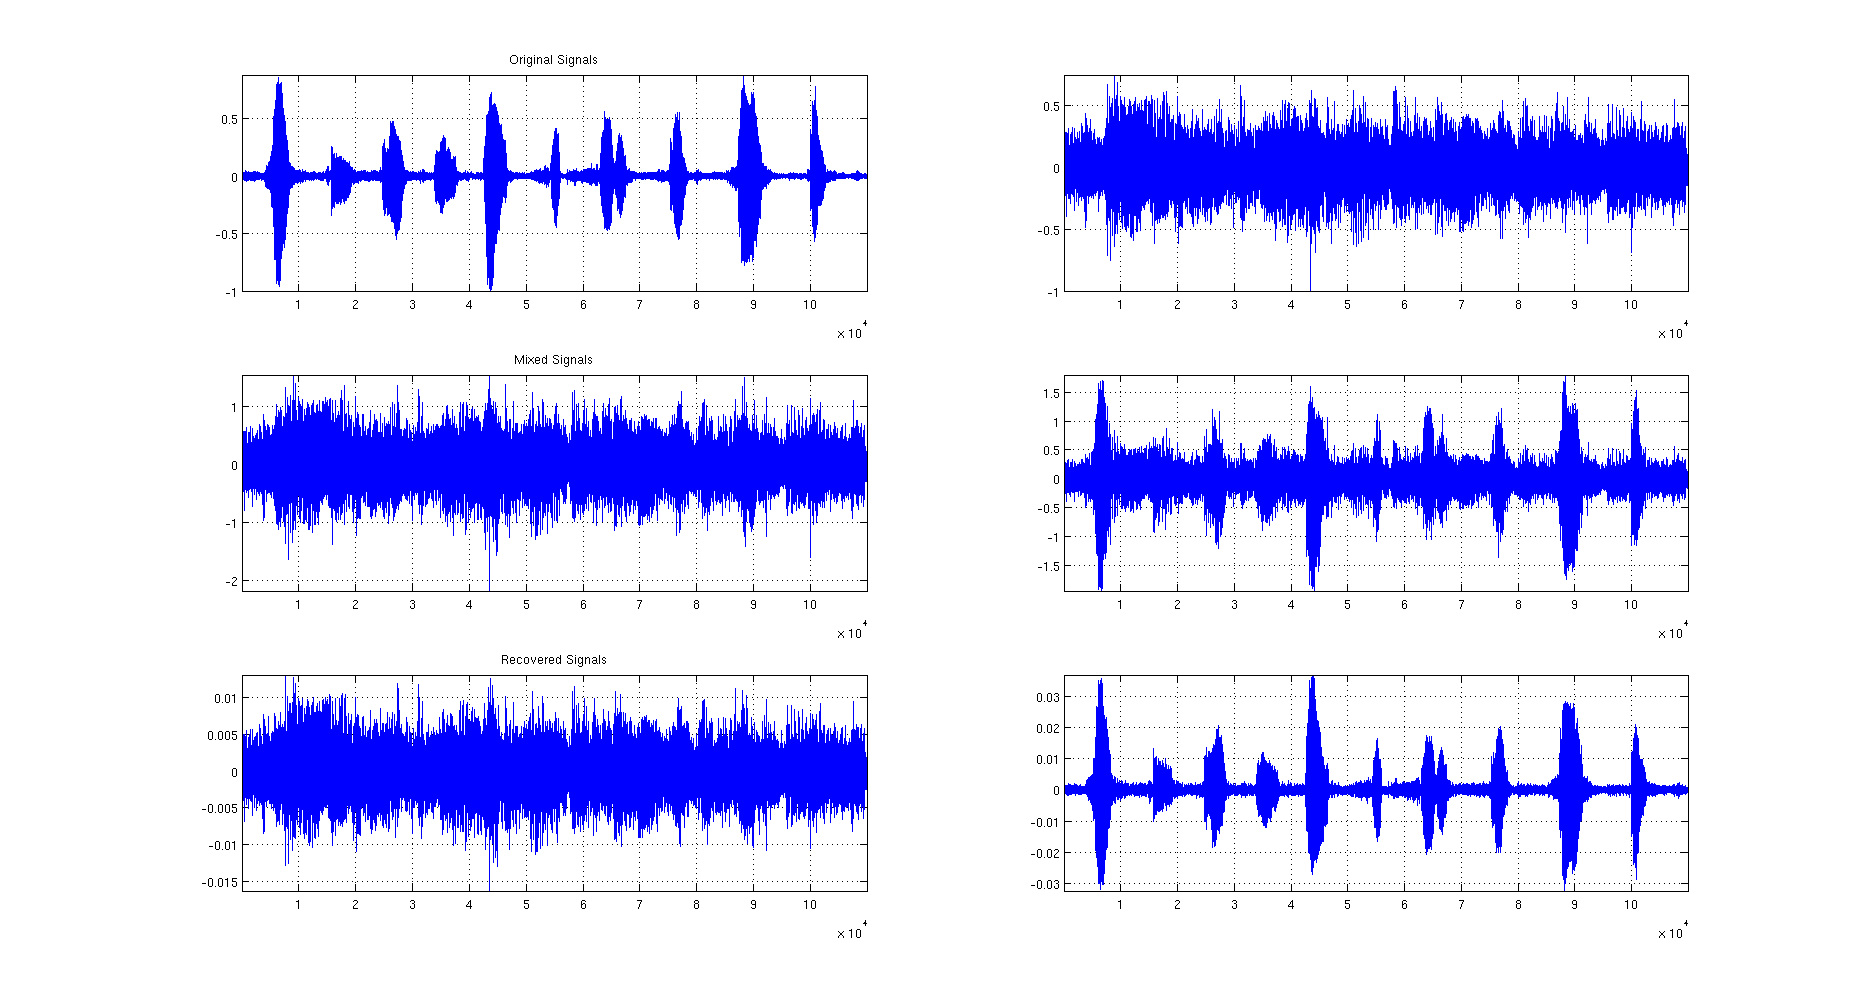
\includegraphics[width = .9\textwidth]{Figures/ica_music_speech}
  \hrule
  \caption{Separating a speech signal (top left) from background music (top right) by ICA. }
\end{figure}



\chapter{Single Sensor Blind Source Separation}\label{ssbss_chap}

Single sensor BSS\footnote{Also called single channel BSS.} is a
particularly important case of the underdetermined BSS problem where the observed
signal consists of only a scalar value at any point in time as if the
source signals were recorded a sole microphone. This presents us with
particular challenges, and we often need to make further assumptions
about the data generating process -- i.e. we need a more complex
generative model.

In this chapter we present  a solution to the single sensor BSS
problem proposed by Roweis (XXXX)\cite{roweis} that relies on a
latent variable model (mixture of gaussians). This metod has two 
phases; a training phase where the mixture models are estimated
one clean recordings of each source. The subsequent inference 
phase where mixed signals are separated rely on two important ideas: an
approximation for determining which source is active at a given time,
and an efficient pruning method to reduce the computational cost
of the model.


% TODO!!
This chapter is structured as follows. Section \ref{timeFreqRep}
provides an introduction to the time-frequency domain signal
representation which is common in most single channel audio separation
models. Section \ref{logmaxapprox} discusses the logmax property
that is fundamental to the inference algorithm. Section \ref{latent_bss}
introduces the key ideas of this chapter. First we review mixture models
in general terms before we look at estimating and doing inference in the 
particular latent variable model at hand. Finally, we briefly discuss an
extended hidden markov model proposed by Roweis, before we illustrate the
method with a few simple examples in Section \ref{ssbss_results}.



\section{Time Frequency Signal Representation}\label{timeFreqRep}


A time frequency representation (TFR) is a redundant signal
representation in comparison to a simple time domain representation that
contains only the amplitude values at given point in time. As seen in
for instance Figure REF, sound signals are often non-stationary,
which indicates that a windowed or short-term analysis is
appropriate. 


\begin{figure}
  \centering
  \hrule
  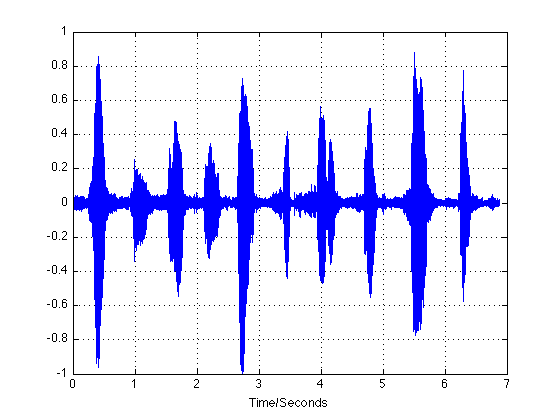
\includegraphics[width = .8\textwidth]{Figures/time_signal}
  \caption{Time domain representation of a male voice counting from
    one to ten.}
  \hrule
\end{figure}



In working with underdetermined blind source separation, we
rely on a redundant signal representation in the time-frequency
domain, rather than the standard representations in the time
domain. Time-frequency representation is advantageous in comparison with a
pure spectral representation as the latter contains no information on
when different components of a signal occur in time. While many
different time-frequency representations exist, our presentation
relies on the \emph{short-term Fourier transform} (STFT).

The time-frequency representation, often called a \emph{spectrogram} produced by the STFT maps the
energies in various parts of the spectrum over the timespan of the
signal. For a low amplitude portion of the signal will have its energy
concentrated in the upper part of the spectrogram and vice versa. This
is illustrated in Figure XX.

Equation \ref{stft} defines the discrete time STFT for the $n$th
segment (which is centered around $m$):

\begin{equation}\label{stft}
  \text{STFT}\{x[n]\}(m,\omega)= X(m,\omega) =\sum_{n = -\infty}^{\infty}
  x[n]\omega[n-m]e^{-i\omega n}
\end{equation}

Here, $\omega$ is a zero centered window function, typically uniform
or gaussian. The window determines which part of the signal $x$ is to
be included in the spectrogram near $m$. In practice, the STFT is
computed using the fast fourier transform (FFT). To better allow for
visualization of the STFT, which is a complex number, the spectrogram
is defined as the squared magnitude of the STFD (Equation \ref{spectrogram}).

\begin{equation}\label{spectrogram}
  \text{spectrogram}\{x[n]\}(m,\omega) = |X(m,\omega)|^2 
\end{equation}

Figure \ref{count_spectrogram} shows a spectrogram represented as a colormap. Here, the abscissa and
ordinate of a point represent time and frequency respectively, while the spectral intensity at the is
color coded with red representing high energy.

%% ANDERS: SKRIV NOE OM TYPISK VINDULENGDE / BROAD vs NARROWBAND SPECTROGRAM

\section{Log Max Approximation}\label{logmaxapprox}

An important observation underlying the inference model discussed in this chapter is the following.
If two signals $s_1(t)$ and $s_2(t)$ are mixed \emph{additively} in the time domain so that 
$x(t) = s_1(t) + s_2(t)$, then the mixture log spectrogram $\log F(x)$ is almost equal to the 
element-wise maximum of the source log spectrograms, that is 
$\log (F(s_1) + F(s_2)) \simeq \max(\log (F(s_1)) + \log (F(s_2))$. The relationship is illustrated in Figure
\ref{logmax_fig}.

\begin{figure}[h!]
  \centering
  \hrule
  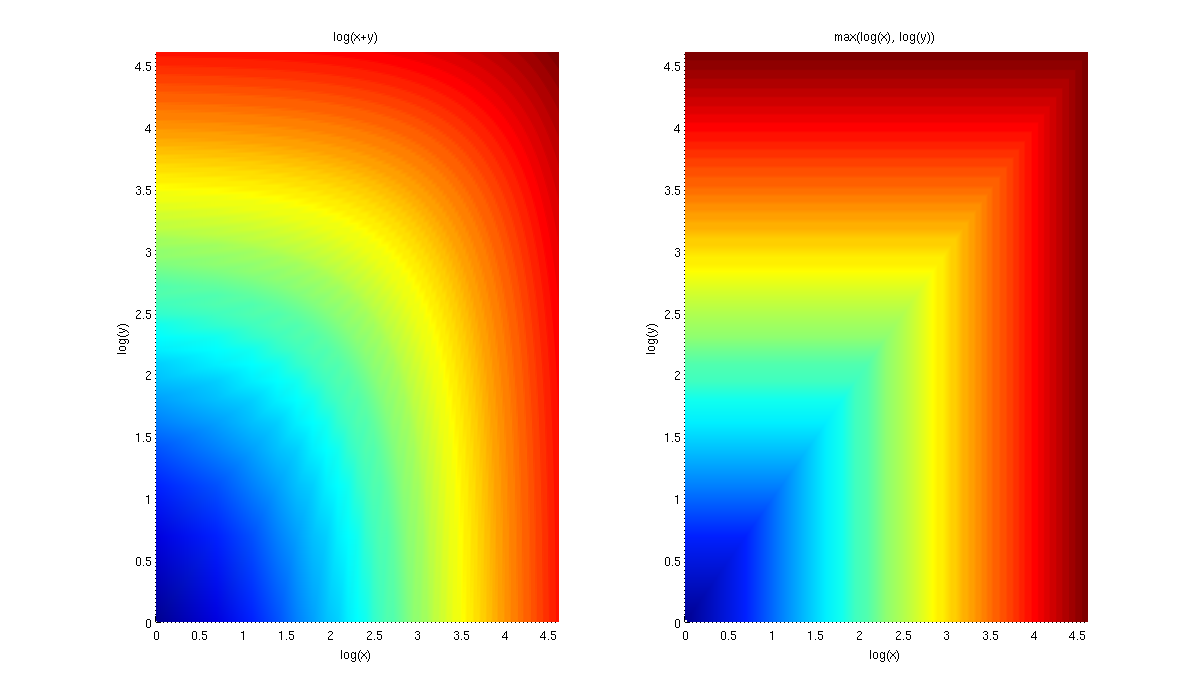
\includegraphics[width = .9\textwidth]{Figures/logmax}
  \hrule
  \label{logmax_fig}
  \caption{Log-max approximation.}
\end{figure}

There is a simple intuition behind this approximation; in the spectral domain, a signal is characterized
by how energy is distributed over different frequency bands, and particular sounds have a ``signature''
according to which frequencies have the highest energies. Hence, if we allow for the assumption that
the signals are more or less independent, \emph{different} signals are likely to have different energy 
distributions at a given point in time. We should also not that the use of logarithms is important here as 
it accentuates the differences between signals.


\section{Latent Variable BSS}\label{latent_bss}

While we are essentially dealing with a \emph{two-level latent variable model}, we follow
Roweis' terminology, adopting the term \emph{factoral-max vector quantizer} or MAXVQ for 
this class of models. This will also provide a ground for discussing the complexity issues
of traditional inference methods as pertains to factorial BSS models, and a proposed solution
to these problems.

We start by looking at gaussian mxiture models in general terms in Section \ref{gmm_general}. 
We then turn to specifying the latent variable model of BSS and briefly describe the estimation 
procedure for this model in Section \ref{generative_model} before we conclude the theoretical
part of this chapter by looking at inference, first by standard methods, and subsequently by a more 
efficient pruning algorithm.

\subsection{Gaussian Mixture Models}\label{gmm_general}
A gaussian mixture model (GMM) is latent variable model that gives a
tractable representation of high-dimensional probability
distribution. Let $Z$ be a multinomial random variable taking on
values $z \in \{1,2,3,...,N\}$ and $\{X_i\}$, $i \in \{1,2,3,...,N\}$
be a set of (multivariate) Gaussian random variables. If $X$ and $Z$
har the joint distribution (\ref{gaussmix_eqn}) then we say $X$ and $Z$
has a gaussian mixture distribution:

\begin{equation}\label{gaussmix_eqn}
  \mathbb{P}(X,Z) = \mathbb{P}(X|Z)P(Z) = \sum_{i = 1}^N
  \Phi(X_i,\mathbf{\mu}_i, \mathbf{\Sigma}_i)Mn_N(Z)
\end{equation}
 
Here, $\Phi(X,\mathbf{\mu}, \mathbf{\Sigma})$ denotes $X$ having a
gaussian distribution with expectation vector $\mathbf{\mu}$ and
covariance matrix $\mathbf{\Sigma})$, and $Mn_N(Z)$ denotes $Z$ having
an $N$-valued multinomial distribution.


A common interpretretation of the gaussian mixture model is for $Z$ to
represent a latent or hidden variable describing the state of a
system, while $X$ is some observable quantity depending on the state
of the system. 

 
\begin{figure}
  \centering
  \hrule
  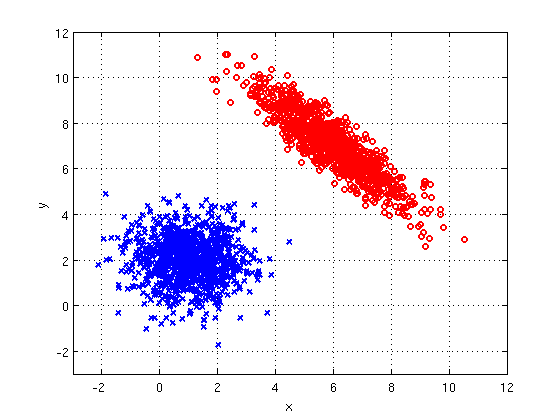
\includegraphics[width = .8\textwidth]{Figures/gaussmix}
  \hrule
  \caption{A mixture of gaussians distribution with two components.}
  \label{gmm_fig}
\end{figure}

Figure \ref{gmm_fig} illustrates a mixture of gaussians distribution with
two components where the component an observation is drawn from is marked
by red circles and blue crosses. Here the two components represent two different 
bivariate distributions with separate means and covariance matrices. A common 
assumption reducing the computational complexity is to estimate a shared covariance
matrix for all components. 

When speaking of a \emph{latent} variable, we refer to the fact that we as observers of
a stochastic process do not know 
whether an observation $x$ is generated from the ``red'' or the ``blue'' distribution. 
It is as if an ``invisible hand'' selects one of the two distributions and then generates
a random number accordingly. 



\subsection{Generative Model}\label{generative_model}

Let $\mathcal{Q} = \{q_1, q_2, .. , q_M\}$ denote the set of speakers\footnote{For 
simplicity, we assume $M=2$.}, and $Q$ be a multinomial random variable over $\mathcal{Q}$, 
$\mathcal{Z}_m  = \{z_1^m, z_2^m, .. , z_N^m\}$ be the set of states for the latent variable 
$Z^m$ for source $m$. Finally, we let $\boldsymbol{X}(t) = (x_1,x_2,...,x_D)$ be an \emph{observed} 
$D$-dimensional frequency vector. The generative model for a given frequency band $d$ is then:

\begin{equation}
  \label{maxvq_eqn}
  \begin{array}{lcl}
    \mathbf{P}(q)   = Mn_M(q) \\
    \mathbf{P}(z|q) = Mn_N^q(z) \\ 
    z^d_{max} = \max_mz_{md} \\
    \mathbf{P}(x_d|z) = \Phi(x^d|z^d_{max},\sigma) \\
  \end{array}
\end{equation}

where $Mn_M(\cdot)$ refers to an $M$-valued multinomial distribution,
and $\Phi(\cdot|\mu,\Sigma)$ the normal distribution. The idea can be
expressed as follows: \emph{Each source $m$ selects a latent variable
  $z$ which in turn produces an intensity vector $\mathbf{x}_m$
  according to the distribution $\mathbb{P}(\mathbf{x}|z)$. The final
  output $\mathbf{x}$ is the elementwise maximum over all vectors
  $\{\mathbf{x}_1, \mathbf{x}_2, ..., \mathbf{x}_M\}$}.


The model is trained in an unsupervised manner by estimating a
gaussian mixture to a training dataset where sources are
separated. More recently, attempts have been made at estimation
directly on mixed signals [REFERANSE]. The canonical training method
used in these models is the expectation maximization (EM) algorithm as
described in appendix [[[REF]]]. 


\subsection{Estimation Procedure - The EM Algorithm}

TODO!
%%%% GENERELT BS OM HVORFOR DET ER VANSKELIG A ESTIMERE MED LATENTE VARIABLER
% + ALGORITME


\subsection{A Generic Inference Procedure}

Having estimated the gaussian mixture models 
corresponding to each one of our sources, we turn to the problem of recovering the set of
orignial signals from the mixture spectrogram $\boldsymbol{S}_{mix}$. Our algorithm in this section
is based on Roweis (REF MAXVQ), but in this step we will ignore the branch-and-bound procedure,
and instead do the inference steps based only on the GMMs.

The approach is an iterative method. Since we make no assumptions on the temporal dynamics of
our signals, we can perform a inference step-by-step, considering each column of the spectrogram
independently. We adopt the following notation: let $\boldsymbol{\Phi}_1 = \{ \mu_1^1,...,\mu_1^N, \Sigma_1 \}$
and $\boldsymbol{\Phi}_2 = \{ \mu_2^1,...,\mu_2^M, \Sigma_2 \} $ denote the GMMs (assuming equal covariance
matrices for all components of each GMM).

Given a single column vector $\boldsymbol{X}$ of the spectrogram, we find the 
most likely component for each GMM:


\begin{equation*}
  \begin{array}{lcl}
    \mu_1^* & = & \arg\max_i \mathbb{P}(\mu_1^i | \boldsymbol{X},\Sigma_1)\\
    \mu_2^* & = & \arg\max_i \mathbb{P}(\mu_2^i | \boldsymbol{X},\Sigma_2)\\
  \end{array}
\end{equation}

As usual, we apply Bayes' rule in estimating the probabilities:

\begin{equation}
  \label{bayes_eqn1}
  \mathbb{P}(\mu_k^i | \boldsymbol{X},\Sigma_k) \propto \mathbb{P}(\boldsymbol{X} | \mu_k^i,\Sigma_k)  
\end{equation}

for each GMM component $k$. Given that the all our mixture components have a multivariate
normal distribution, it is simple to show that the following\footnote{We can interpret (Equation \ref{mahala})
geometrically as selecting the nearest component to the observed data under the \emph{Mahalanobis} 
metric.} holds true for the right hand side of (Equation \ref{bayes_eqn1}).

\begin{equation}\label{mahala}
  \mathbb{P}(\boldsymbol{X} | \mu_k^i,\Sigma_1) \propto 
  (\boldsymbol{X} - \mu_k^i)^T\Sigma_k^{-1}(\boldsymbol{X} - \mu_k^i)
\end{equation}

Knowing most likely components of each source given the observed data, we subsequently turn to 
computing the \emph{masking signal} for each frequency band, ie. for each element of $\boldsymbol{X}$. 
This masking signal is computed for every source $i$, and takes the value $1$ if source $i$ is the
maximum over all sources at the given frequency band/timestep pair and zero otherwise. 



\subsection{An Improved Pruning Method for MAXVQ Inference}\label{prune}

The purpose of the inference part of the model is computing the most
likely sequence of source/gmm component combinations given the
observed data. In the previous section we discussed a naïve method
for doing this that applies standard machine learning principles.
For large datasets, this method quickly becomes computationally
intractible.

To amend this problem reducing time complexity of the inference procedure,
Roweis [[xxx]] describes a branch-and-bound methodbased on
estimating an upper bound on the log likelihood of the latent variables
given the observed data.

For source/latent variable combination $(m,k)$, given each observation
vector, $\mathbf{x}$, we compute the following bound.

\begin{equation}\label{bound}
  B_{m,k} = -\frac{1}{2}\sum_d \max(x^d - v_m^d,0)^2 - \frac{D}{2}\log|D|-\log \pi_m
\end{equation}

Next, let $z_m^{*} = \arg \min B_{m,k}$, and let $l^{*}$ be
the log likelihood associated with $z_m^{*}$. For all sources $m$, we
eliminate latent variables $k$ such that $B_{mk}<l^{*}$. For the
remaining source/latent variable combinations, we evalutate the log
likelihood by the model specified in \ref{maxvq_eqn}. If a new lower
bound is discovered, we reiterate the pruning procedure over the remaining
source/component combinations with the new
bound, otherwise, we compute log likelihoods until all remaining are 
evaluated.



\begin{figure}[!htpb]
  \begin{lstlisting}[frame=single]
% Variables:
gmms        % List of GMM(comp_1,...,comp_N)
spectrogram % d x T matrix
bounds      % List of best bound for 
            % (source m / speaker k)
masks       % Mask matrix of dimension d x T x 2. 
            % Entry corresponds to active 
            % (source/component)
minIdx      % index of best component
            % for each source
for t = 1:T
  X = spectrogram(t)

  % Initial bound estimate
  bounds = list()
  for m = 1:length(gmms)
    for k = 1:NComponents(gmms(m))
      bounds(m,k) = computeBound(X, gmms(m,k))

  % Max log likelihood for each source
  for m = 1:length(gmms)
    minIdx(m) = argmin(bounds(m))
    l0(m) = logLikelihood(bounds(m,minIdx(m)))
  
  % Reduction
  while length(bounds) > 0
    for m = 1:length(gmms)
      for k = 1:NComponents(gmms{m})
        if bounds(m,k) < l0
          % Delete observation from list
          bounds = bounds - bounds(m,k)
        else
          l1 = logLikelihood(bounds(m,k))
          if l1 < l0
          l0 = l1
  
  % Set masks   
  for i = 1:d
    sourceIdx = argmin(l0(d))
    masks(d,t) = (sourceIdx, minIdx(sourceIdx))
  \end{lstlisting}
  \caption{Pseudocode for MAXVQ algorithm.}
  \label{maxvq_pseudo}
\end{figure}



\section{Factorial Hidden Markov Model for BSS}\label{fhmm}

We will now describe the factoral HMM for blind source separation as
put forward by Roweis in a two signal setting. We adopt the following
notation: for each timestep $t \in \{1,2,3,...,T\}$, $\mathbf{X}_t$
denotes the $M$-dimensional spectral vector of power spectral
intensities over the finite set of frequency values $\mathcal{F}$. We
note that while the set of frequencies are discrete, the intensities
$x_{it}$ are real-valued, hence we adopt a real valued emission
model, as discussed later. 


\begin{figure}\label{count_spectrogram}
  \centering
  \hrule
  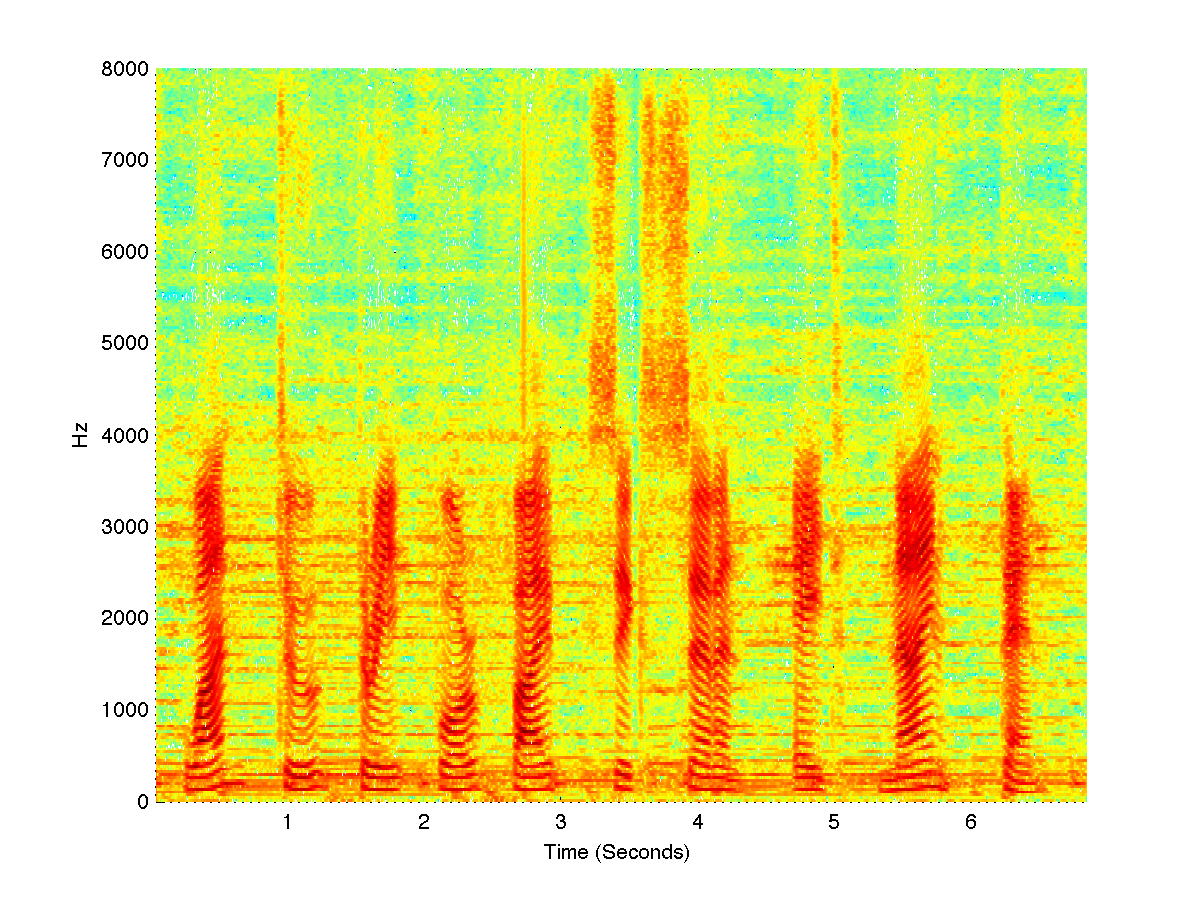
\includegraphics[width = .9\textwidth]{Figures/spectrogram_count}
  \hrule
  \caption{Spectrogram of male voice counting from one to ten.}
\end{figure}


The FHMM is essentially a supervised learning method, and the learning
process consists in estimating a separate HMM based on separate (clean) recordings of the
particular source. That is to say, the learning part consists entirely
in learning a probability model of each source. 

For a given source, the training phase then consists in
training a HMM with a discrete (latent) state space $\mathcal{Z}$, and
a continuous emission distribution $\mathbf{P(X|Z)}$. The emissions
model will produce intensity vectors $\mathbf{X}_t$ as described in
the preceding paragraph.



\subsection{Initialization}

The factoral hidden markov model consists of one HMM per speaker which
is trained on separate non-mixed training data for each source. 

The initialization of the FHMM training consists in estimating the
emission probabilities $P(X|Z)$ (see figure, lag figur). While Roweis
operates with a finite state model for the latent variables, the
observable variables are real valued intensities. This indicates that
a mixture model may be appropriate in the inital estimate of the
emission model (vis til andre artikler med samme greier ). 

We follow Roweis in estimating a Gaussian mixture model with a single
shared covariance matrix $\mathbf{\Sigma}$. For a spectrogram with $N$ frequency bands,
our approach is to estimate a GMM with $k$ $N$-dimensional components
or latent variables. The mean vector $\mathbf{\mu}_i\in\mathbb{R}^N$ for
each component $i$ represents the expected intensity (power spectral
density value) in each frequency band given that the system is in
state $i$. The pair $(\{\mathbf{\mu}_i\}, \Sigma)$ then forms the initial
parametrization of the emissions model.




\subsection{Separation}

Next, consider the problem of recovering the orignial
sources\footnote{For simplicity, we will here frame the problem in
  terms of two sources.} $\mathbf{S} =
\{S_1, S_2\}$ given the observed sequence $\{\mathbf{Y}(t)\}$, $t \in \{1,2,3,...,T\}$ which we
take to be spectral vectors as discussed above. As before, we let
$z_k(t)$, $i \in \{1,2\}$ denote the value of the latent variable for
each HMM. 

A key question in the separation process is how the observable signal
generated by full FHMM relates to the observable values for each of
the underlying HMMs. This question adresses a property of the
\emph{data generating model}, and must reflect properties of the
physical system we are trying to model. In the case of auditory
signals, Roweis argues for model whereby the observed value equals the
maximum value of the observable values $\mathbf{X}_k(t)$ of the
underlying HMMs with an additive gaussian noise:


\begin{equation}
  \mathbf{Y}(t) = \Phi(\{\mathbf{X}_1(t), \mathbf{X}_2(t)\}^{+}, \Sigma)
\end{equation}

For a further discussion on the rationale behind the log-max
approximation, see [REFERANSER].




\section{Results}\label{ssbss_results}

To illustrate the methods outlined in this chapter, we return to our base case signals consisting
of a voice counting from one to ten in English, and a music clip, both lasting approximately 8 seconds as
seen in figure \ref{music_count}. The sampling frequency for both signals is $16,000$Hz.

\begin{figure}\label{music_count}
  \centering
  \hrule
  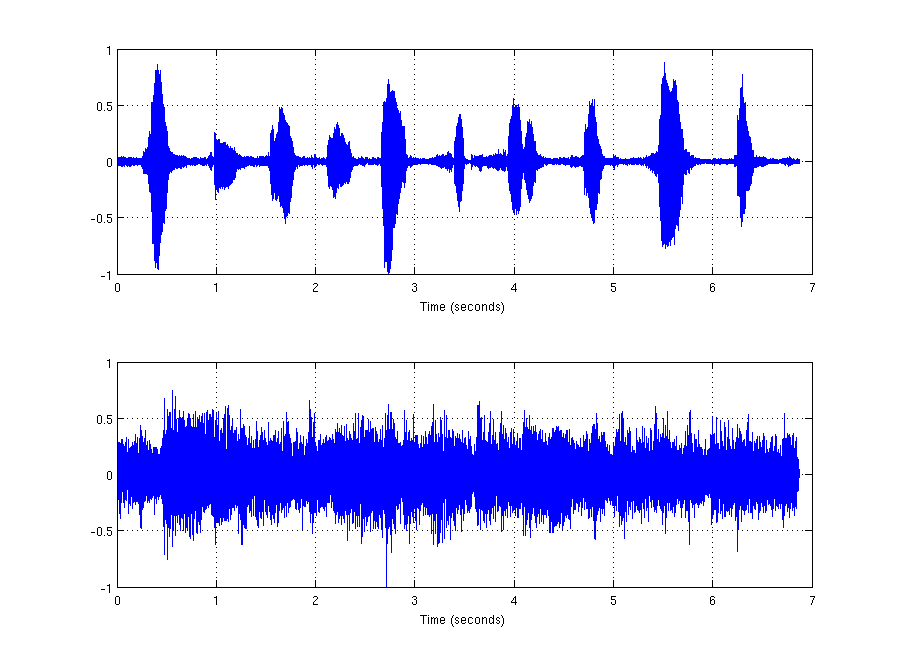
\includegraphics[width = .8\textwidth]{Figures/music_count}
  \hrule
  \caption{Time domain plot of speech (top) and music (bottom).}
\end{figure}

In our experiment in this section we have split the data in half (one training and one test set) 
The is are preprocessed by constructing
one spectrogram per source with Hamming windows of length 512 so that the final matrix of spectral intensities
has $257$ frequency bands, with $4539$ observations each.

From visual inspection of the spectrograms and the temporal plots, it seems that the voice signal is ``richer''
than the music, and that it probably needs more GMM components to be represented properly. We therefore fitted
a model with $256$ components for the voice signal and $128$ for the music\footnote{In Roweis, an experiment is 
conducted where a speech GMM is trained with $512$ components and a ``noise'' GMM has only $32$.}. 


\begin{figure}\label{spect_testset}
  \centering
  \hrule
  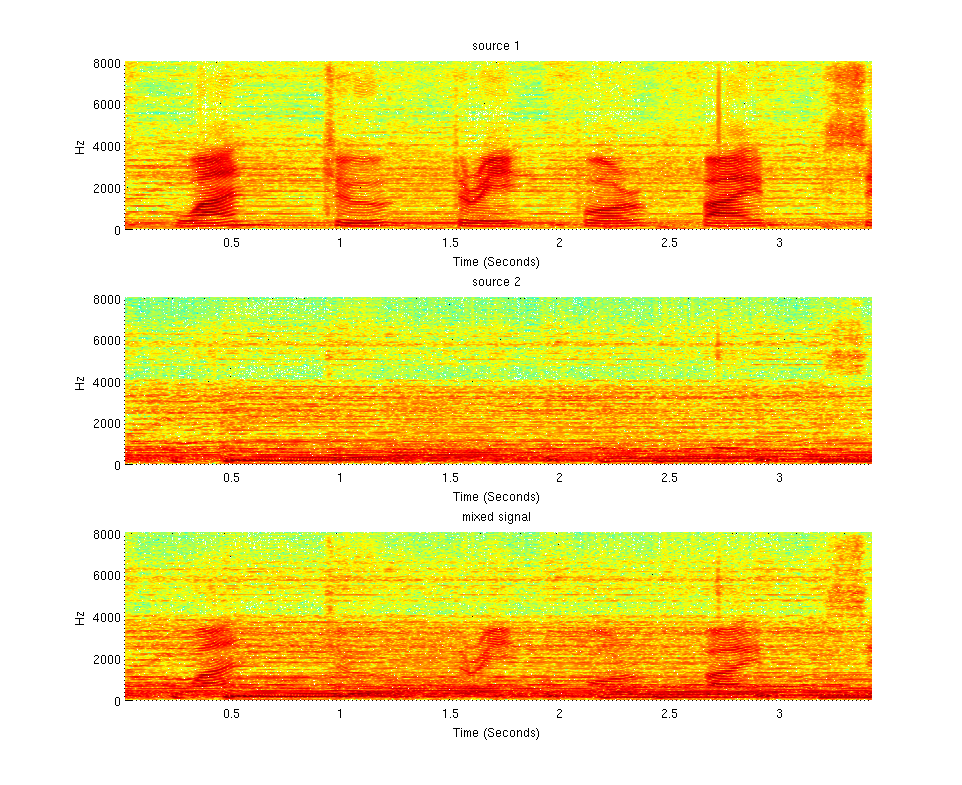
\includegraphics[width = .9\textwidth]{Figures/spectrograms_test}
  \hrule
  \caption{Spectrograms for test data.}
\end{figure}

Top to bottom, Figure \ref{spect_testset} shows spectrograms of the two sources of test set prior to mixing,
and the spectrogram of the mixture from a linear time domain superposition of the two sources in 
the lower spectrogram. 
We see that the second and third utteance in the lowermost spectrogram has is almost ``gone'' due to the 
contamination from the music, whereas we would expect the algorithm to perform reasonably well in recovering
the other utterances which are still quite visible in the mixtures. 

Figures \ref{voice_result}-\ref{spec} shows the recovered voice and music signals for the mixture in 
the lowermost plot in Figure \ref{spect_testset}. While it is hard to appreciate the performance of the 
of the algorithm juding from just a set of spectrograms, we can distinguish some important features that 
are apparent. 

\begin{itemize}
\item The second and third utterance of the speaker which was close to invisible in the mixture spectrogram is now visible in Figure \ref{recovered_voice}.
\item In the recovered voice spectrogram, we still see the markings of the most distinct utterances (1,3,5).  
\end{itemize}




\begin{figure}\label{voice_result}
  \centering
  \hrule
  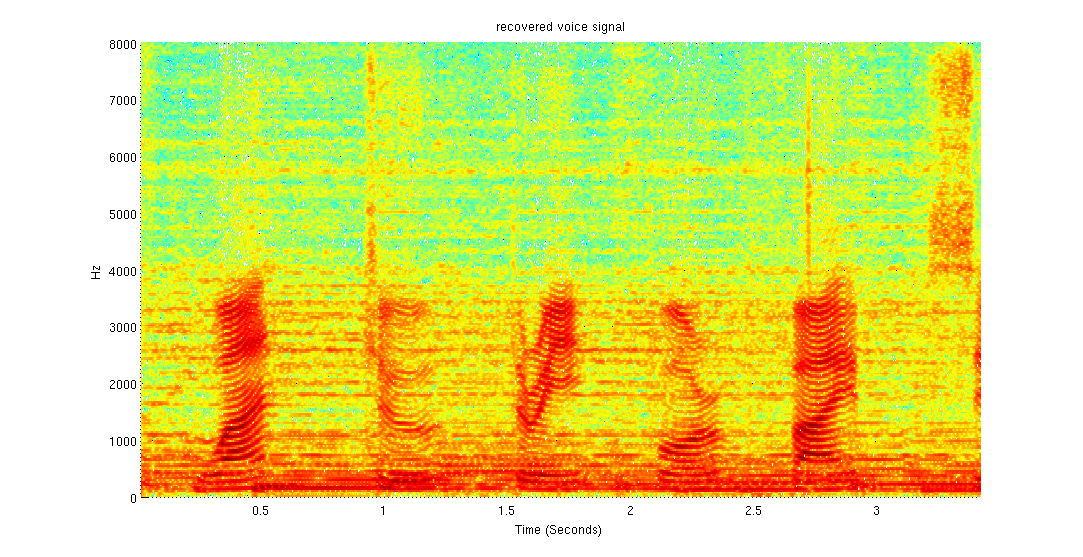
\includegraphics[width = .9\textwidth]{Figures/recovered_voice}
  \hrule
  \caption{Spectrogram for recovered voice signal.}
\end{figure}

\begin{figure}\label{music_result}
  \centering
  \hrule
  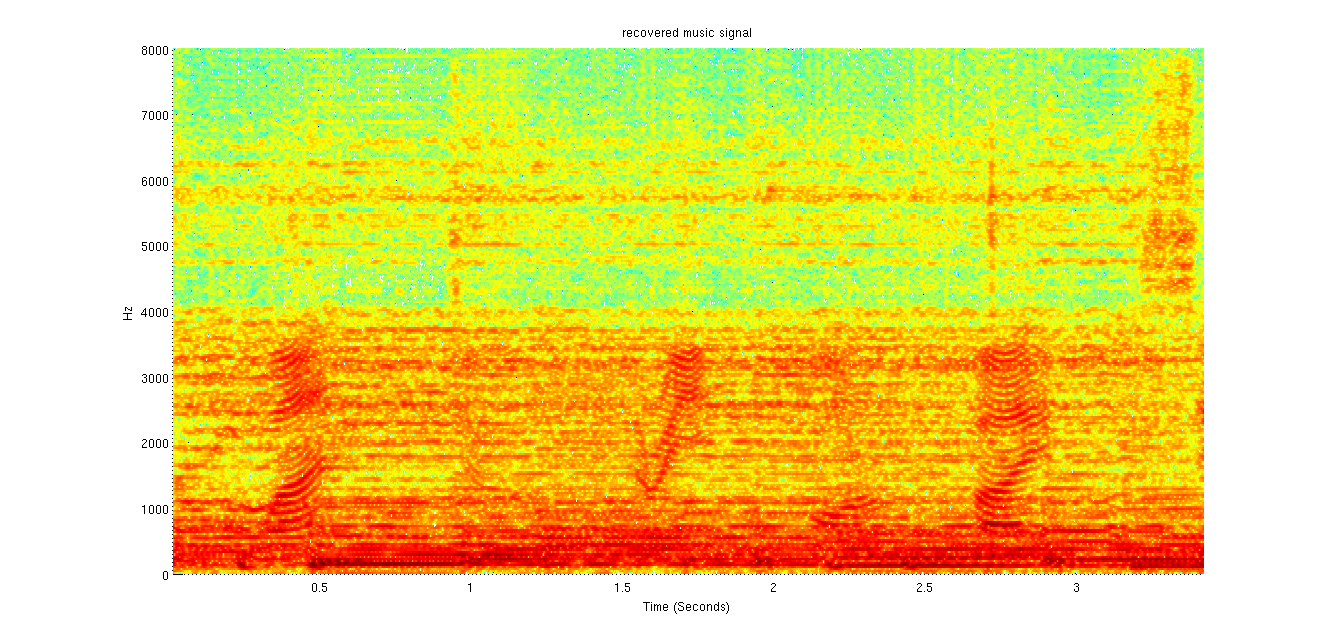
\includegraphics[width = .9\textwidth]{Figures/recovered_music}
  \hrule
  \caption{Spectrogram for recovered music signal.}
\end{figure}





Another point worthwhile mentioning is the complexity of this method. Whereas ICA on the same signals completes
in a matter of seconds, the MAXVQ algorithm takes several minutes. That being said, there is a clear potential
for increasing MAXVQ performance through parallelization as each time step of the inference algorithm is 
processed independently.






\chapter{Conclusion and Further Study}

This report has studied three conceptually different approaches to blind source separation. While conventional 
\emph{principal component analysis} is arguably the simplest and most well-understood method, it is also a useful
background in understanding \emph{independent component analysis} as both these algorithms perform separation
through a de-correlating projection. ICA is also a well-established technique, but there is still on-going
research in developing new ICA-based methods, for instance in handling underdetermined BSS. 

Factoral blind source separation models are a much less developed research area than ICA. An important reason 
for this has been computational complexity. However, improvements made to these methods such as the pruning
method discussed in Section \ref{prune} along with hardware improvements make these models more tractable. 


This report has attention to the assumptions behind the methods discussed in this paper, and how
one would expect these assumptions to impact performance in actual separation tasks. An important extension
of this would be constructing precise measures of such performance. The common format for reporting results 
on separation tasks is through visual representations, either spectrograms or time domain visualizations. This
does of course provide some information but, it is still hard to determine quality through visually inspecting
the differences between an unmixed and a recovered signal - in particular if we are to compare different 
methods using different test data.

Since so little research has been done in constructing appropriate performance measures, to be able to 
differentiate between different methods will in practice require \emph{listening} to the results of 
actual implementations on a given test set. A challenge to future research would therefore be to construct
a framework for doing comparative studies to rigorously determine the relative merits of different methods.

%% \section{Hidden Markov Models}\label{hmm_appendix}
%% %% Ref Norvig
%% A hidden markov model (HMM) is a probabilistic model relating two sequences of
%% discrete random variables $\mathcal{S} = \{S_1, S_2, ..., S_T\}$ and
%% $\mathcal{X} = \{X_1, X_2, ..., X_T\}$. We will refer to
%% $\mathcal{S}$ as the \emph{source} or \emph{hidden} variable, and
%% $\mathcal{X}$ as the \emph{observed} variable. Often, we assume there
%% is some causal relationship whereby the hidden variable affects the
%% observable, but this does not need be the case. 

%% A HMM consists of two probabilistic statement; the \emph{transition}
%% model:

%% \begin{equation}
%% \mathbb{P}(S_t|S_{t-1}, S_{t-2},...,S_1)
%% \end{equation}


%% and the \emph{sensor} or \emph{observation} model:

%% \begin{equation}
%% \mathbb{P}(X_t|S_t, S_{t-1}, X_{t-1}, ...,
%% S_1, X_1)
%% \end{equation}


%%  The order of a markov model is the number of realizations
%% of $\mathcal{S}$ conditioned on in the transition model. In order to
%% make HMMs computationally tractable, we often operate with 1st order
%% markov models:

%% \begin{equation}\label{1st_order_markov}
%%   \mathbb{P}(S_t|S_{t-1}, S_{t-2},...,S_1)  =  \mathbb{P}(S_t|S_{t-1})
%% \end{equation}

%% This can be stated as as ``the future being conditionally independent of
%% the past given the present''. Another common simplification is known as the \emph{markov sensor model assumption}:


%% \begin{equation}
%%   \mathbb{P}(X_t|S_t, S_{t-1}, X_{t-1}, ...,
%%   S_1, X_1) = \mathbb{P}(X_t|S_t)  
%% \end{equation}

%% The sensor markov assumption states that the sensor is independent of
%% everything else given the current value of the hidden variable.


\begin{thebibliography}{99}

\bibitem{comon94} Comon, P. (1994). 
``Independent Component Analysis: a new concept?'', 
Signal Processing, 36(3):287–314

\bibitem{bellSejnowski95} Bell, A.J. and Sejnowski, T.J. (1995).,
``An information maximization approach to blind separation and blind deconvolution'', 
Neural Computation, 7, 1129-1159

\bibitem{pearlmutterParra}Pearlmutter, B. A. and Parra, L. C.(1996),
``A Context-Sensitive Generalization of ICA''. 

\bibitem{hyvarinen2001}Hyvarinen A (2001),
``Independent Component Analysis'',
Neural Computing Surveys, Neural Computing Surveys, vol 2.

\bibitem{bach} Bach, F.R. and Jordan, M.I. (2004),
``Blind One-Microphone Speech Separation: A Spectral Learning
  Approach''.

\bibitem{fastICA}Hyvärinen, A. (1999),
``Fast and Robust Fixed-Point Algorithms for Independent Component
  Analysis''. 
IEEE Transactions on Neural Networks 10(3):626-634, 1999.

\bibitem{roweisOneMic}Roweis, Sam T.(2001).
``Neural Information Processing Systems 13'' (NIPS'00).
pp. 793-799
  
\bibitem{davies2007}Davies, M.E. and James, C.J. (2007).
``Source separation using single channel ICA'',
Signal Process., vol. 87, no. 8, pp. 1819–1832, 2007.

\bibitem{cardoso98}Cardoso, J. L.(1998),
``Multidimensional Independent Component Analysis'',
Proceedings of ICASSP 1998.

\bibitem{mijovic2010} Mijovic, B. De Vos, M.,  Gligorijevic, I.,
  Taelman, J. and Van Huffel, S. (2010),
``Source Separation From Single-Channel Recordings by Combining
  Empirical-Mode Decomposition and Independent Component Analysis'',
IEEE Transactions on Biomedical Engineering, vol. 57, no. 9, September 2010

\bibitem{VargaHMMDecomp}Varga, A. P., and R. K. Moore. 
``Hidden Markov model decomposition of speech and noise"
Acoustics, Speech, and Signal Processing, 1990. ICASSP-90., 1990 International Conference on. IEEE, 1990.

\bibitem{pearson1901}{Pearson, K. (1901). ``On Lines and Planes of Closest Fit to Systems of Points in Space". Philosophical Magazine 2 (6): 559–572.}

\bibitem{Pham}{Pham, D. T. and Garat, P. (1992) ``Blind Separation of Mixture of Independent Sources Through a Maximum Likelihood Approach'', Proc. EUSPICO, pp. 771-774.}

\bibitem{norvig_russel}{Russell, S. and Norvig, P. (XXX). ``Artificial
    Intelligence: A Modern Approach''. XXXX}


\end{thebibliography}








\end{document}

